\documentclass[12pt]{article}

\usepackage{pdflscape}
\usepackage[margin=0.8in]{geometry}
\usepackage{titling}
\usepackage{graphics} %Required for diagrams
\usepackage[hidelinks]{hyperref}
\usepackage{color}
\usepackage{framed}
\usepackage{epsfig}
\usepackage{epstopdf}

\begin{document}

\begin{titlepage}
	\begin{center}
		
		\begin{figure}[t]
			\centering
			
\includegraphics[width=350px]{images/UP_Logo.png}
		\end{figure}
		
		% Title
		\textsc{\large Project Tender} \\ 
		\vspace{2cm}
		\textbf{\Huge Project: RMB's Data Lake} \\ 
		\textsc{\large Client: RMB} \\ 
		\vspace{2cm}
		\textbf{\Huge Team: Team Name } \\ 
		
		%\begin{minipage}{0.4\textwidth}s
		\begin{flushright} \large
			Armand Pieterse \emph{u12167844} \newline
			Kgomotso Sito 		\emph{u12243273} \newline
			student name		\emph{uXXXXXXXX} \newline
			Sphelele Malo 	\emph{u12247040} \newline
			\end{flushright}
		%\end{minipage}
		\textsc{\small Department of Computer Science, University of Pretoria}
		
		\vfill
		
	Here's a link to \href{https://github.com/SpheMalo/COS-301-Main-Project.git}{GitHub}.\\
	\url{https://github.com/SpheMalo/COS-301-Main-Project.git}

	\vfill

	{\large \today}		
		
		
	\end{center}
\end{titlepage}


\newpage
\tableofcontents

\newpage
\listoffigures

\newpage

\section{Vision and scope}

\subsection{Project Background}

\subsection{Project vision}

\subsection{Project scope}

\newpage
\section{Application requirements and design}
\par{This section discusses for each module of the Figbook system the functional requirements
as well as the process designs for the use cases and the domain models which must be maintained
within persistent storage by that module.
}

\subsection{Authentication}

\subsubsection{scope}
\par{This module takes care of everything involving the users account. This includes functionality like logging in and out of the system, editing of user accounts etc. Further description is provided in the use cases below}

\begin{figure}[h]
	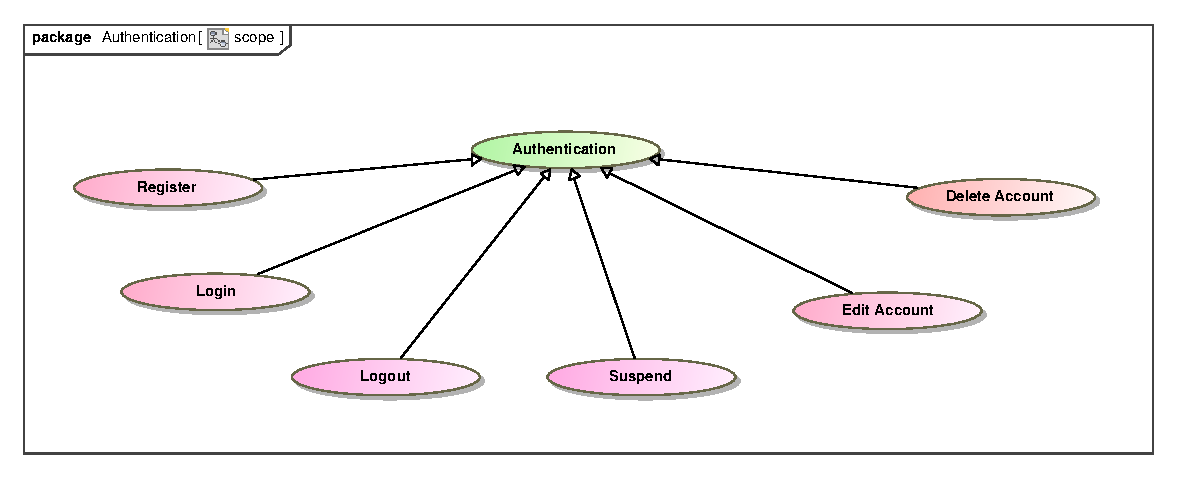
\includegraphics[scale=0.9]{epsImages/Authentication/AuthenticationScope.eps}
	\caption{Scope for authentication module}
\end{figure}

\newpage
\subsubsection{Use Cases}

\begin{enumerate}

\item \textbf{registerAccount  – priority: critical } 
This use case creates  a user account that gets persisted to database.

\textbf{Service Contract:}

\begin{figure}[h]
		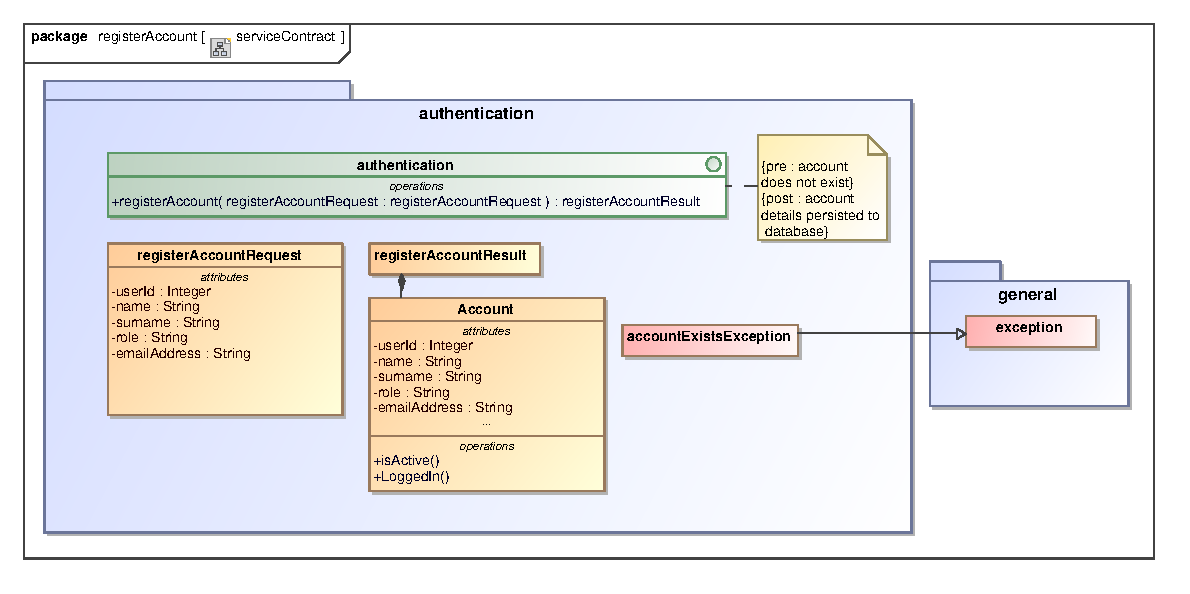
\includegraphics[scale=0.9]{epsImages/Authentication/serviceContract.eps}
		\caption{Service contract for registering new user account}
\end{figure}

\newpage
\item \textbf{Login - priority: critical}
This use case allows a user to log into an existing account.

\par{\textbf{Service Contract} The service contract for the login service is shown in figure below.}
\begin{figure}[h]
		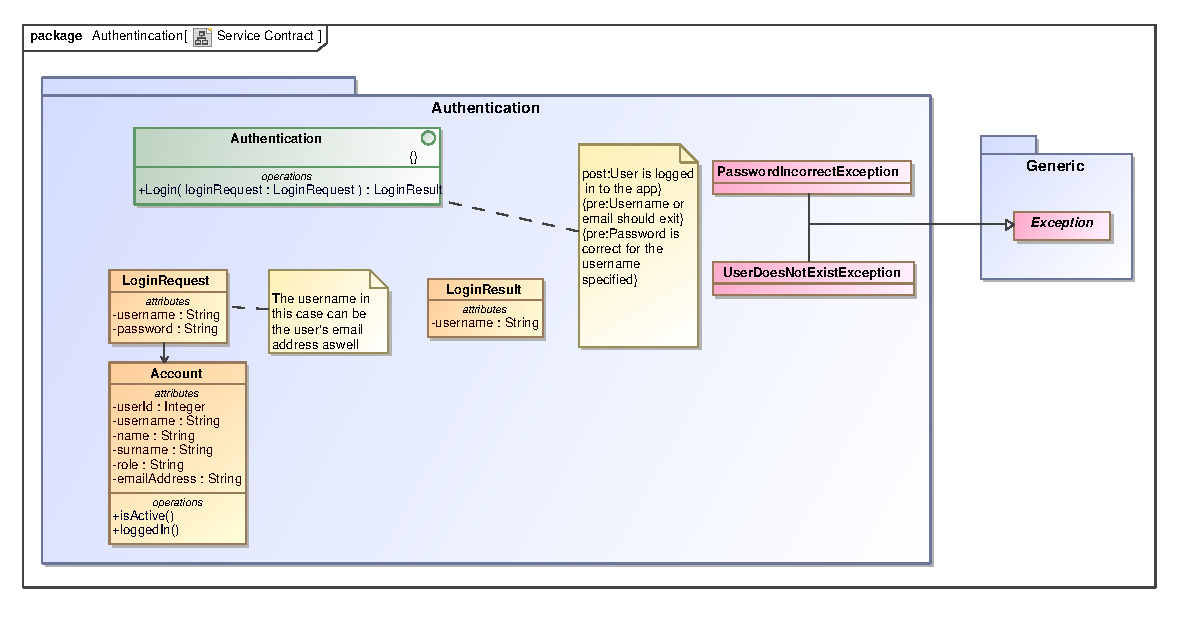
\includegraphics[scale=0.9]{epsImages/Authentication/LoginServiceContract.eps}
		\caption{Service contract for logging into a user account}
\end{figure}

\item \textbf{Logout - priority: important} \\
This use case allows a user to log out of the system safely. \\ \\

\textbf{Service Contract:}
\begin{figure}[h]

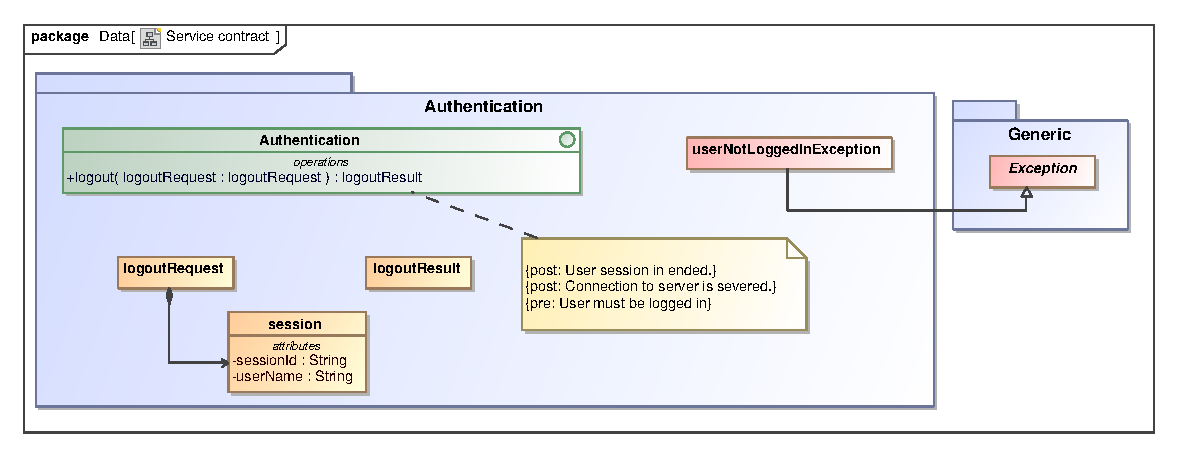
\includegraphics[scale=.9]{epsImages/Authentication/logoutServiceContract.eps}
\caption{Service contract for logging a user out of the system}
\end{figure}

\newpage
\item \textbf{editAccount - priority: important}
	\par{This allows a user to make changes to their profile details. They will be allowed to edit the details they added when creating the account.}\\ \\
	
	\textbf{Service Contract:}\\
	\begin{figure}[h]
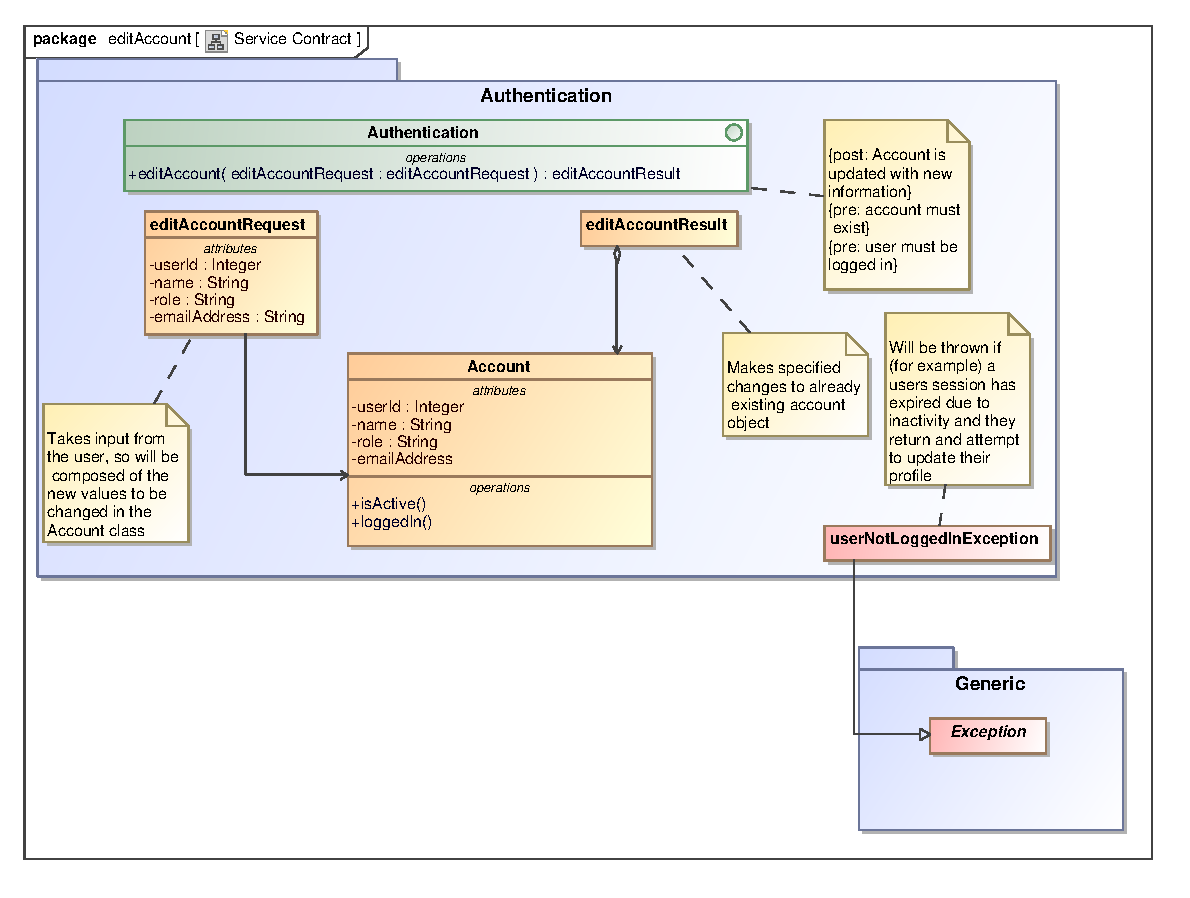
\includegraphics[scale=0.9]{epsImages/Authentication/editAccountServiceContract.eps}
\caption{Service contract for editing a users account}
\end{figure}

\newpage
\item \textbf{deleteAccount  – priority: important} 
This use case creates  a user account that gets persisted to database.

\textbf{Service Contract:}

\begin{figure}[h]
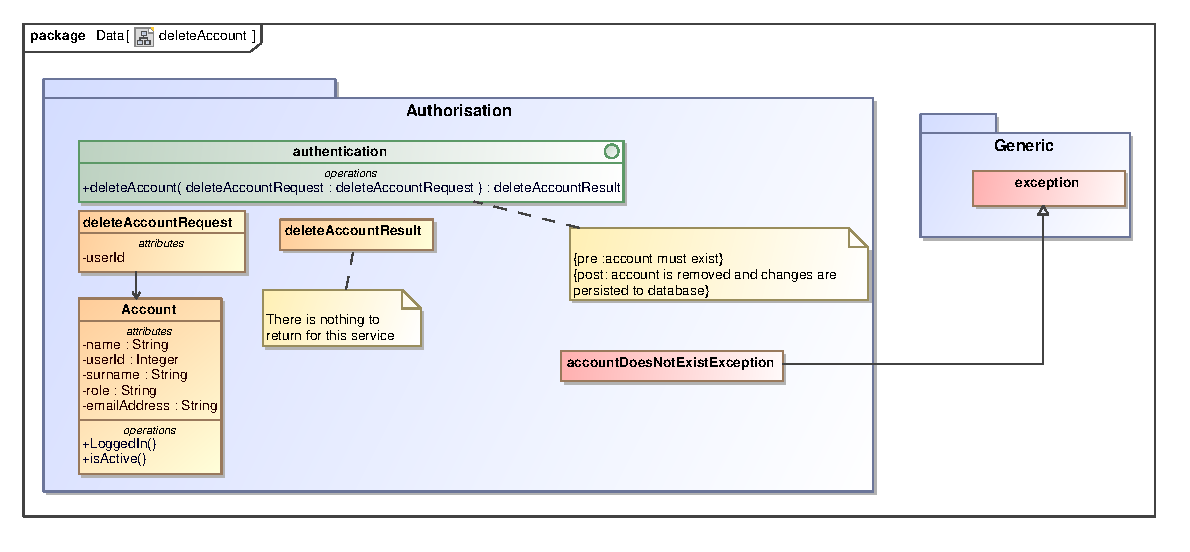
\includegraphics[scale=0.9]{epsImages/Authentication/deleteAccount.eps}
\caption{Service contract for deleting a users account}
\end{figure}

\newpage
\item \textbf{SuspendAccount - priority: important}\\
\par{This use case allows the system administrator to suspend a users account for any reason he/she may see as appropriate. A suspended account bars the user from logging in and/or using the account until the administrator lifts the suspension.}\\ \\

\textbf{Service Contract:}

\begin{figure}[h]
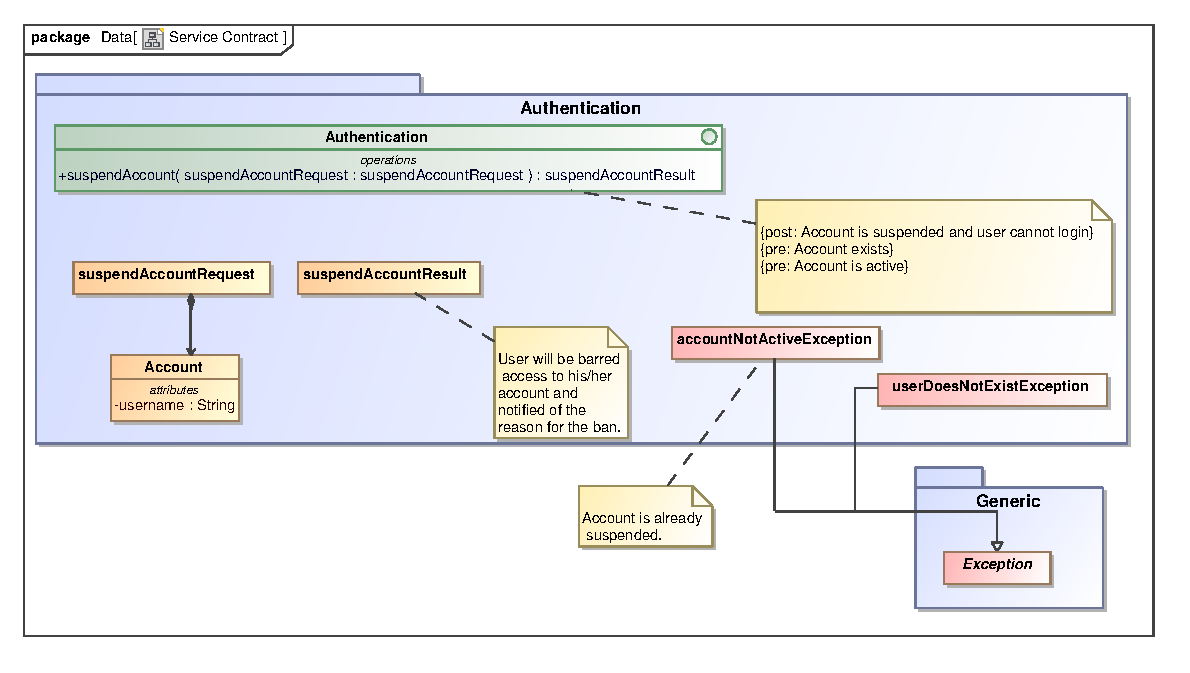
\includegraphics[scale=0.9]{epsImages/Authentication/suspendServiceContract.eps}
\caption{Service contract for suspending a users account}
\end{figure} 
\end{enumerate}

\newpage
\subsubsection{Domain Model}
\par{ The Authentication module will keep Account objects in the database. Any part of the system that checks for user authorisation will check against the account table to see if that particular user has authorisation to do whatever it is they are attempting to do. }

\begin{figure}[h]
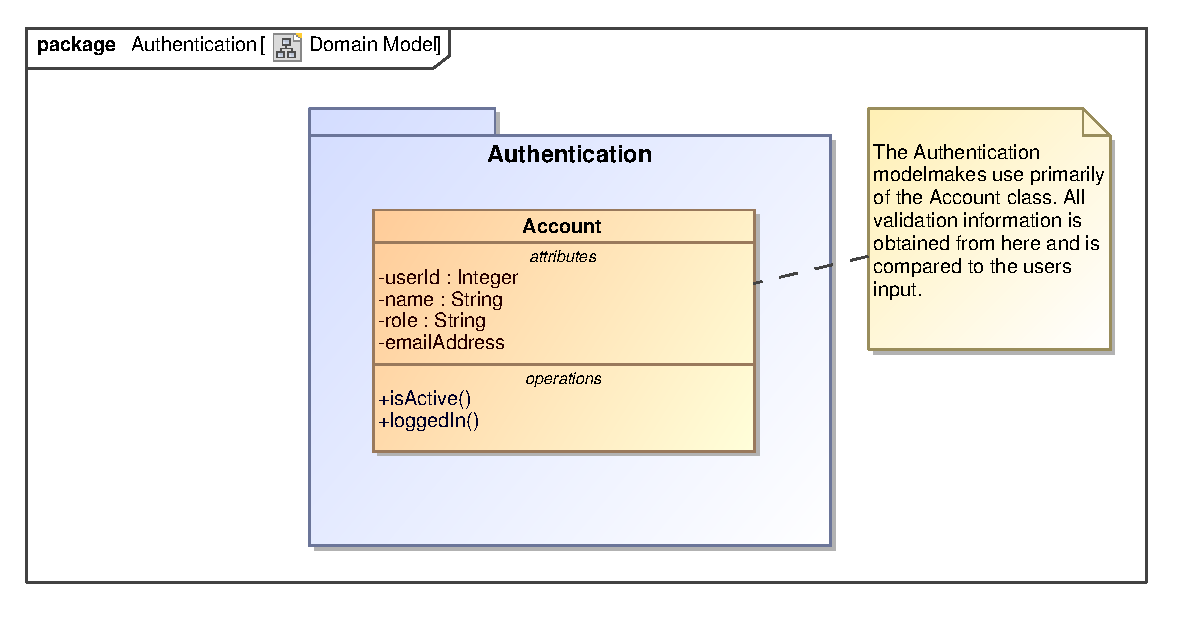
\includegraphics[scale=0.9]{epsImages/Authentication/domainModel.eps}
\caption{Domain model of Authentication module}
\end{figure}

\newpage

\subsection{Manuscript Management}

\subsubsection{Scope}
\par{This section provides the detailed service contracts and activity diagrams(where needed) for the use cases offered by the Manuscript Management module.
It's services includes all the needed functionality to create, read, evaluate, edit and to send it to the next role in the life-cycle of creating a quality book.}

\begin{figure}[h]
	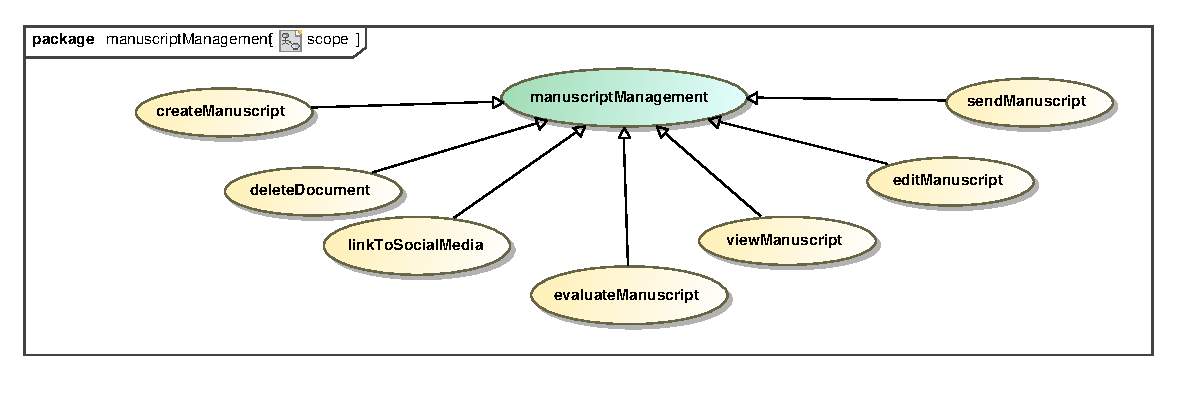
\includegraphics[height=200px, width=500px]{epsImages/ManuscriptManagement/scope.eps}
	\caption{Scope for manuscript management module}
\end{figure}

\newpage
\subsubsection{Use Cases}
\begin{enumerate}
\item \textbf{Create Manuscript - priority: critical}

\par{This use case allows an author to create a new project, by creating a new manuscript. The author will be able to give the manuscript a name(title) and specify the privacy setting on it. There may be one or multiple authors collaborating on a manuscript.
A manuscript's title should be unique.}\\

\textbf{Service Contract:}

\begin{figure}[h]
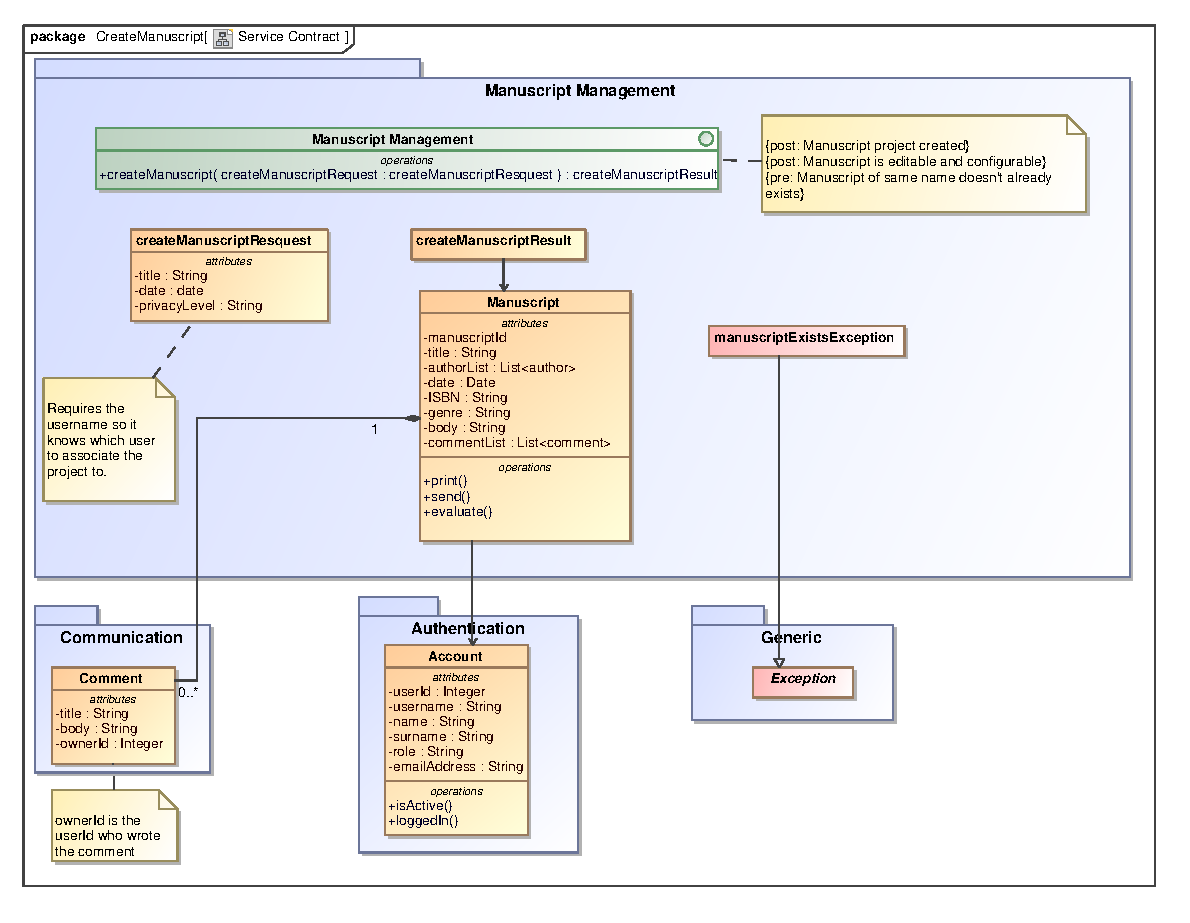
\includegraphics[height=330px, width=500px]{epsImages/ManuscriptManagement/createManuscriptServiceContract.eps}
\caption{Service contract for creating a new project (manuscript)}
\end{figure}

\newpage
\item \textbf{Delete Manuscript – priority: important}
\par{This use case removes an existing manuscript. The pre-conditions are enforced (raising the appropriate exception should they not be met) and the manuscript of interest is deleted and changes are persisted through to database.}

\textbf{Service Contract:} 


\begin{figure}[h]
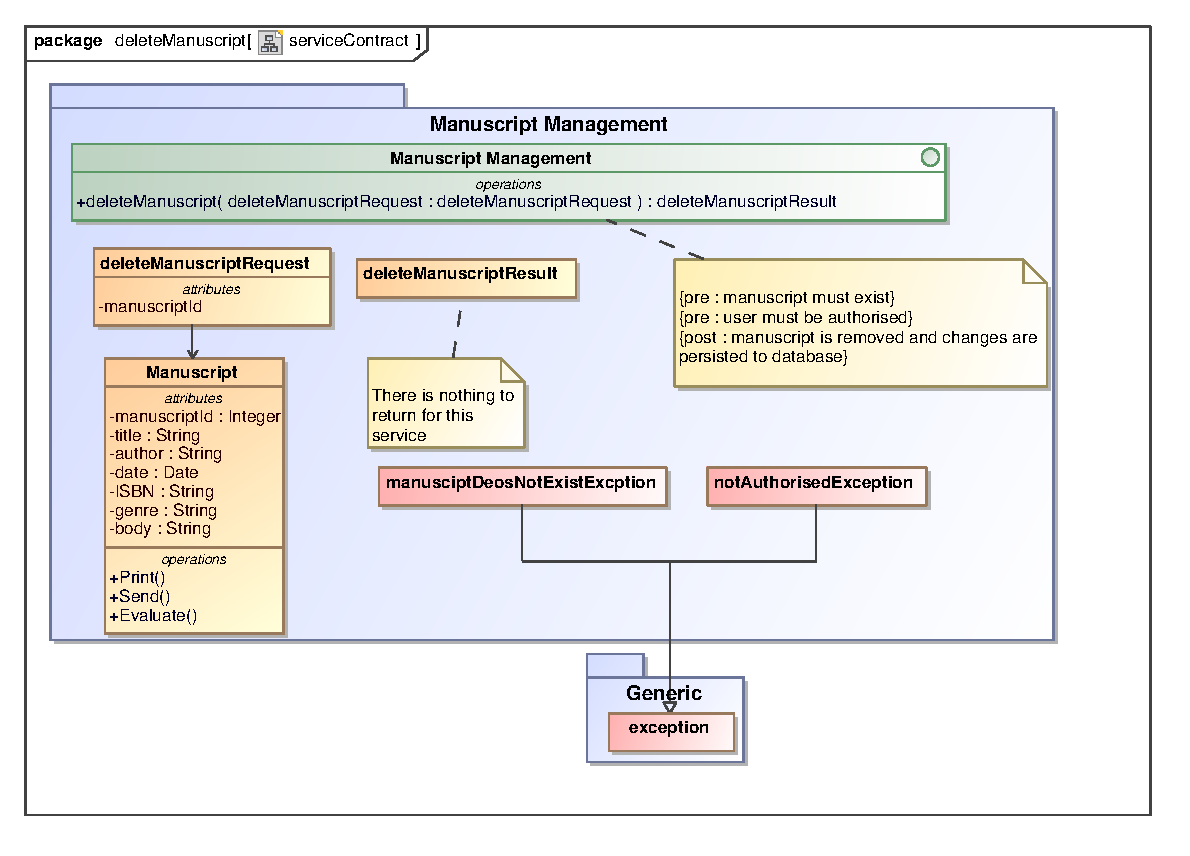
\includegraphics[height=330px, width=500px]{epsImages/ManuscriptManagement/deleteManuscript.eps}
\caption{Service contract for deleting a  project (manuscript)}
\end{figure}

\newpage
\item \textbf{Link To Social Media – priority: important}\\
\par{This use case links a project(manuscript) to a social media of choice if conditions are met and creates an automated post on that social media.}

\textbf{Service Contract:}

\begin{figure}[h]
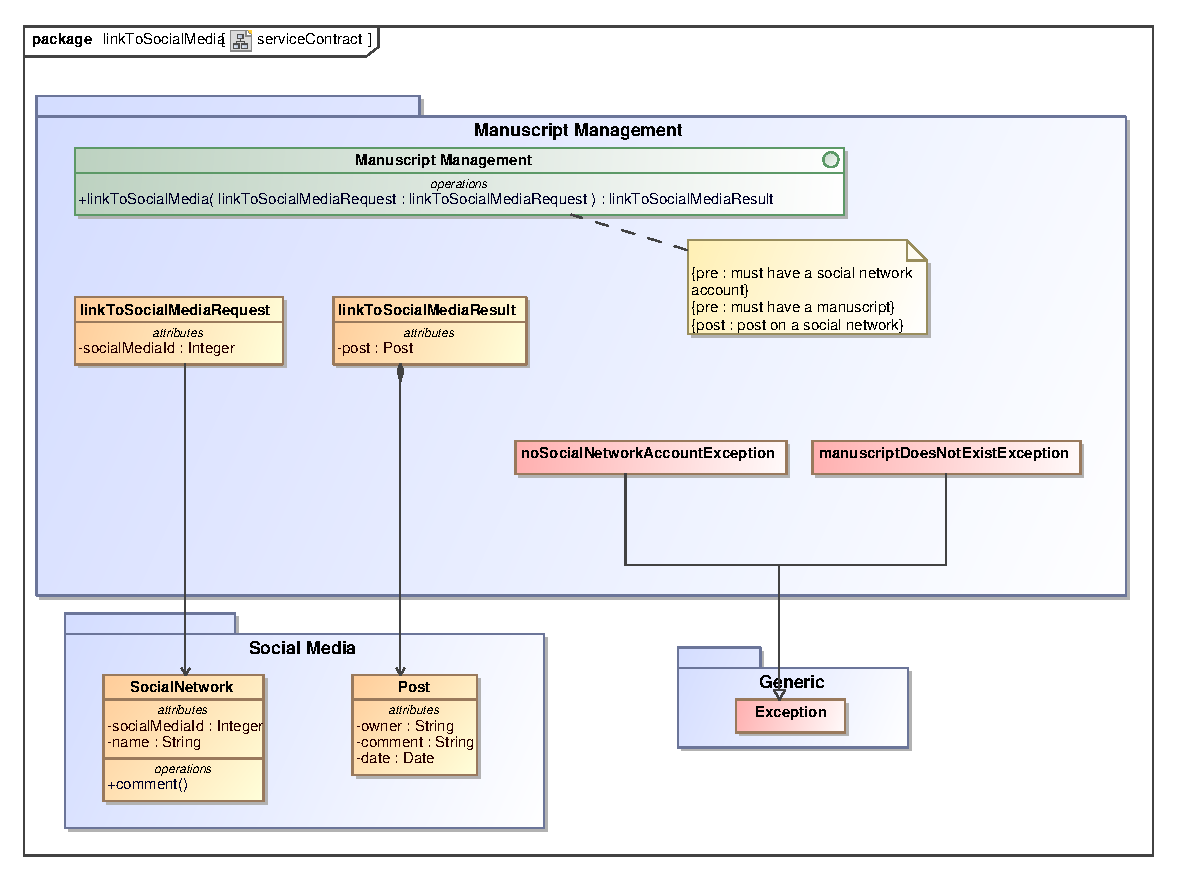
\includegraphics[height=330px, width=500px]{epsImages/ManuscriptManagement/linkToSocialMedia.eps}
\caption{Service contract for linking a  project (manuscript) to a social network}
\end{figure}

\newpage

\item \textbf{Edit Manuscript – priority: critical}
\par{This use case which allows one to edit a manuscript if authorized and afterwards changes are persisted to database.}

\textbf{Service Contract:}

\begin{figure}[h]
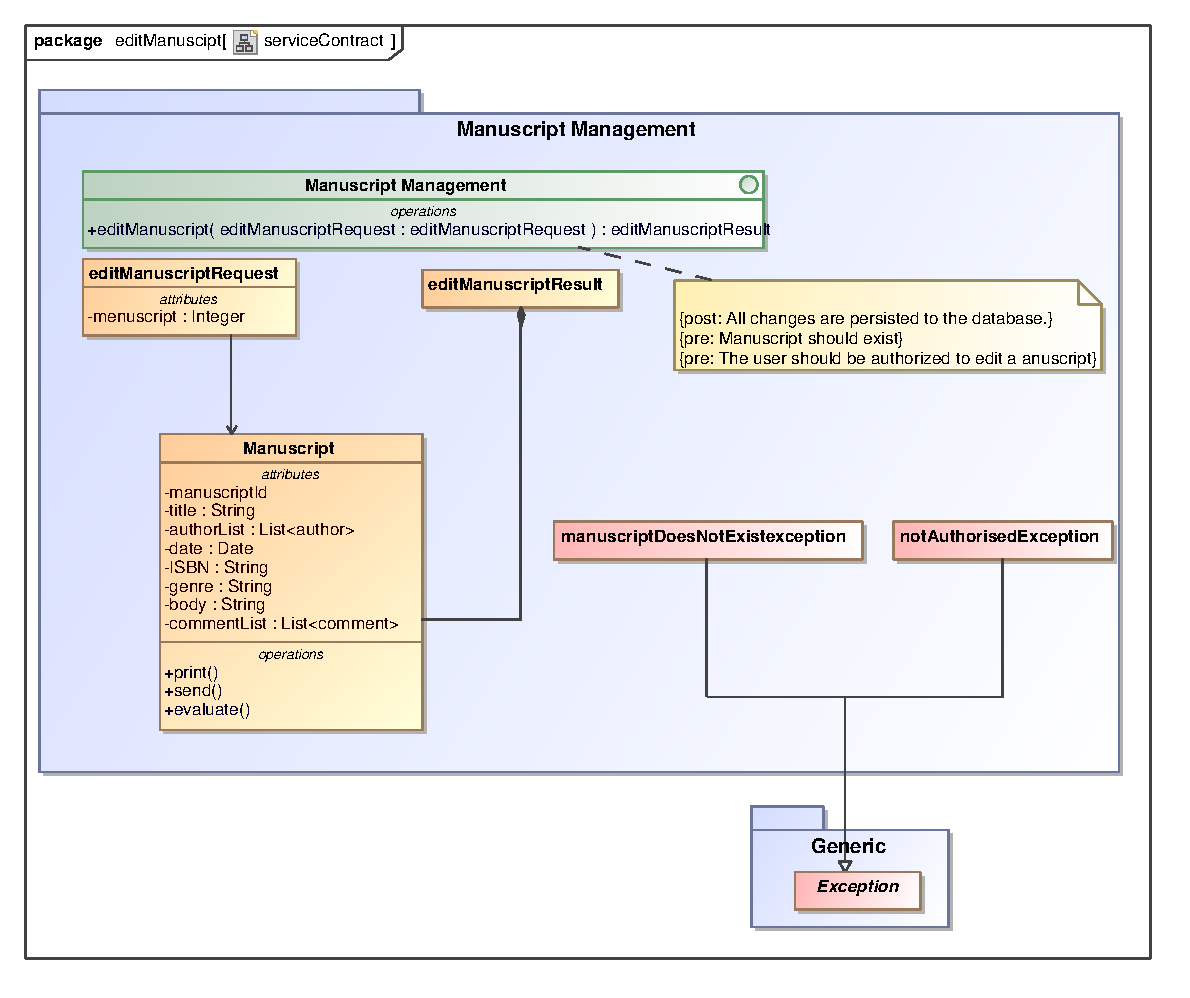
\includegraphics[height=330px, width=500px]{epsImages/ManuscriptManagement/editManuscript.eps}
\caption{Service contract for editing a  project (manuscript)}
\end{figure}
\newpage

\item \textbf{Evaluate Manuscript - priority: critical}
\par{This use case allows an agent or an editorial to evaluate the manuscript and to give the according feedback to the author, such as a comment or editorial letter.}

\textbf{Service Contract:}

\begin{figure}[h]
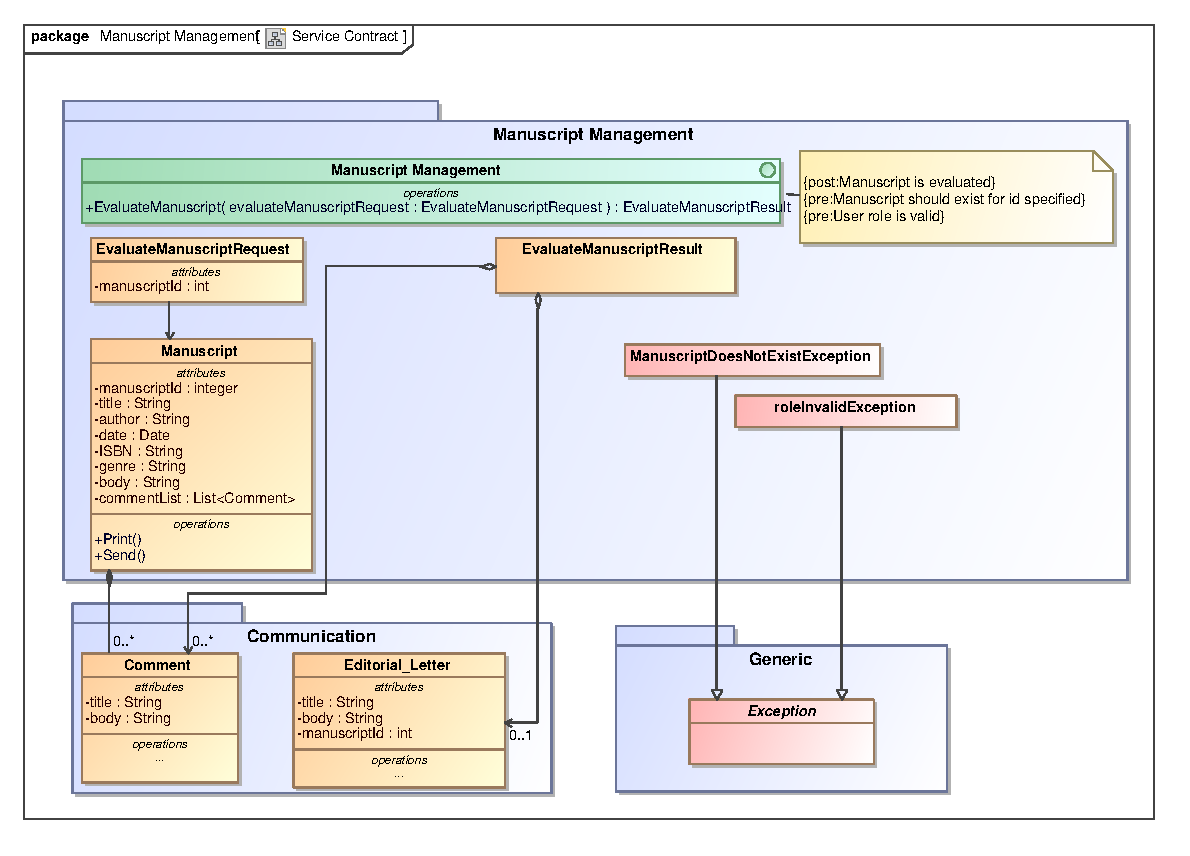
\includegraphics[height=240px, width=500px]{epsImages/ManuscriptManagement/EvaluateManuscript.eps}
\caption{Service contract for evaluating a manuscript}
\end{figure}

\textbf{Process Specification (Activity diagram):}
\begin{figure}[h]
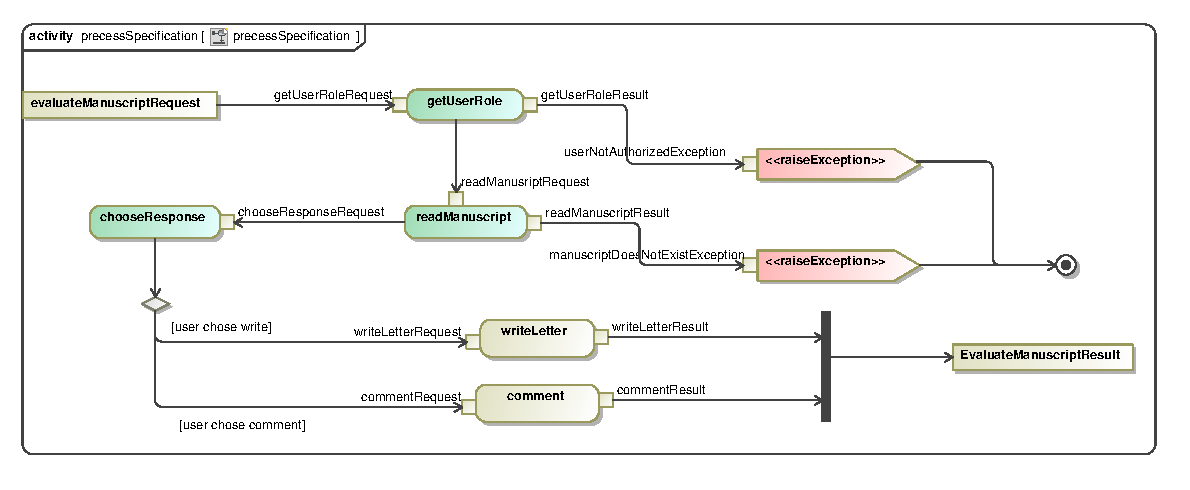
\includegraphics[height=200px, width=500px]{epsImages/ManuscriptManagement/EvaluateActivity.eps}
\caption{Process Specification for evaluating a manuscript}
\end{figure}

\newpage
\item \textbf{Read Manuscript - priority: critical}
\par{The use case grants access to users to view/read a manuscript, under the conditions that the user is authorized and that the manuscript still exists.}

\textbf{Service Contract:}

\begin{figure}[h]
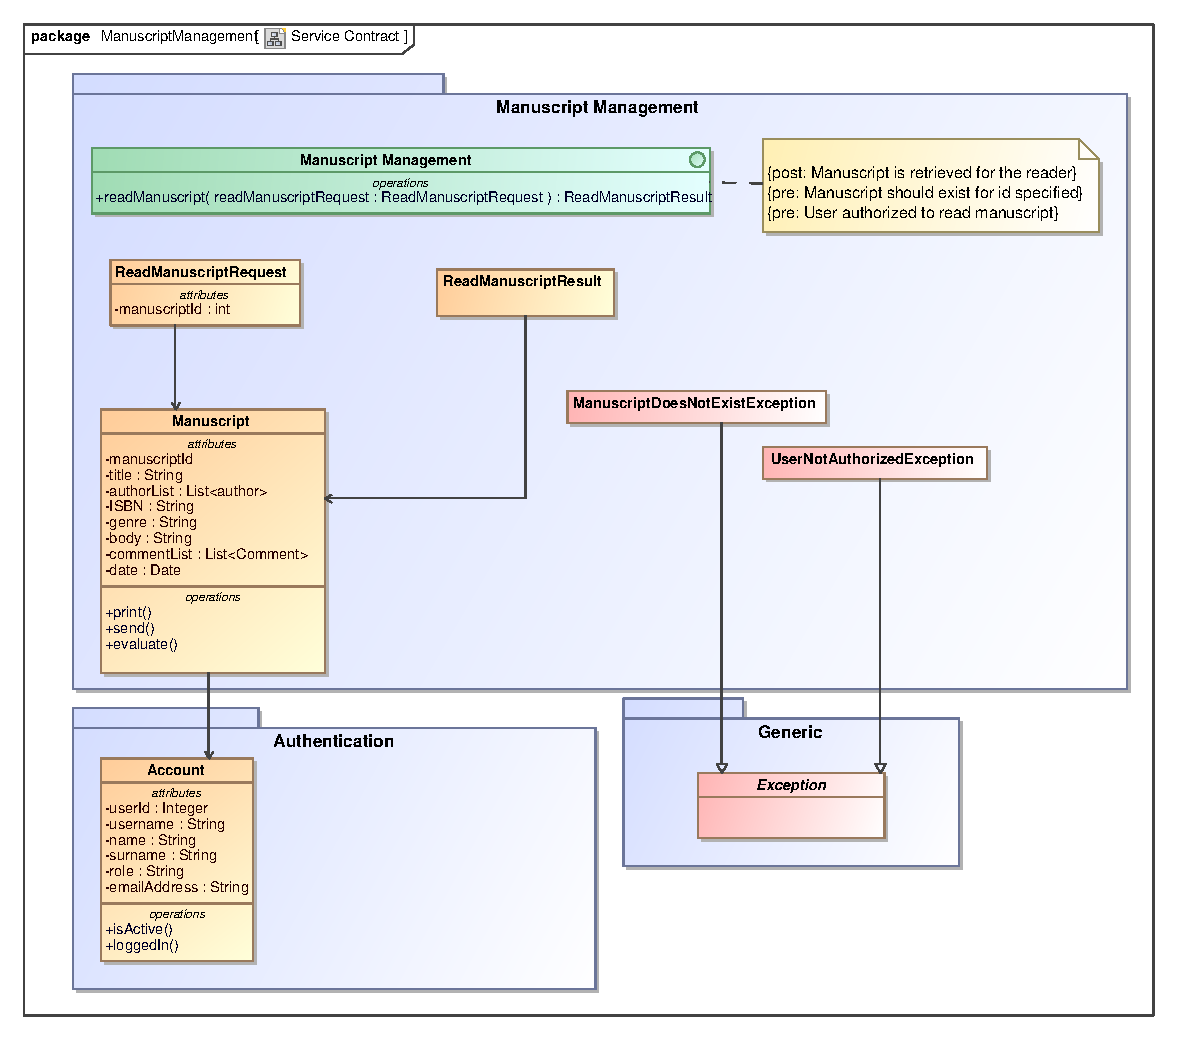
\includegraphics[height=330px, width=500px]{epsImages/ManuscriptManagement/ReadManuscript.eps}
\caption{Service contract for reading a manuscript}
\end{figure}

\newpage
\item \textbf{Send Manuscript - priority: critical}
\par {This use case allows a user link another user on the system to the manuscript. This allows the recipient to access it and, depending on the privileges afforded by the owner of the manuscript, be able to read/modify it.}

\textbf{Service Contract:}

\begin{figure}[h]
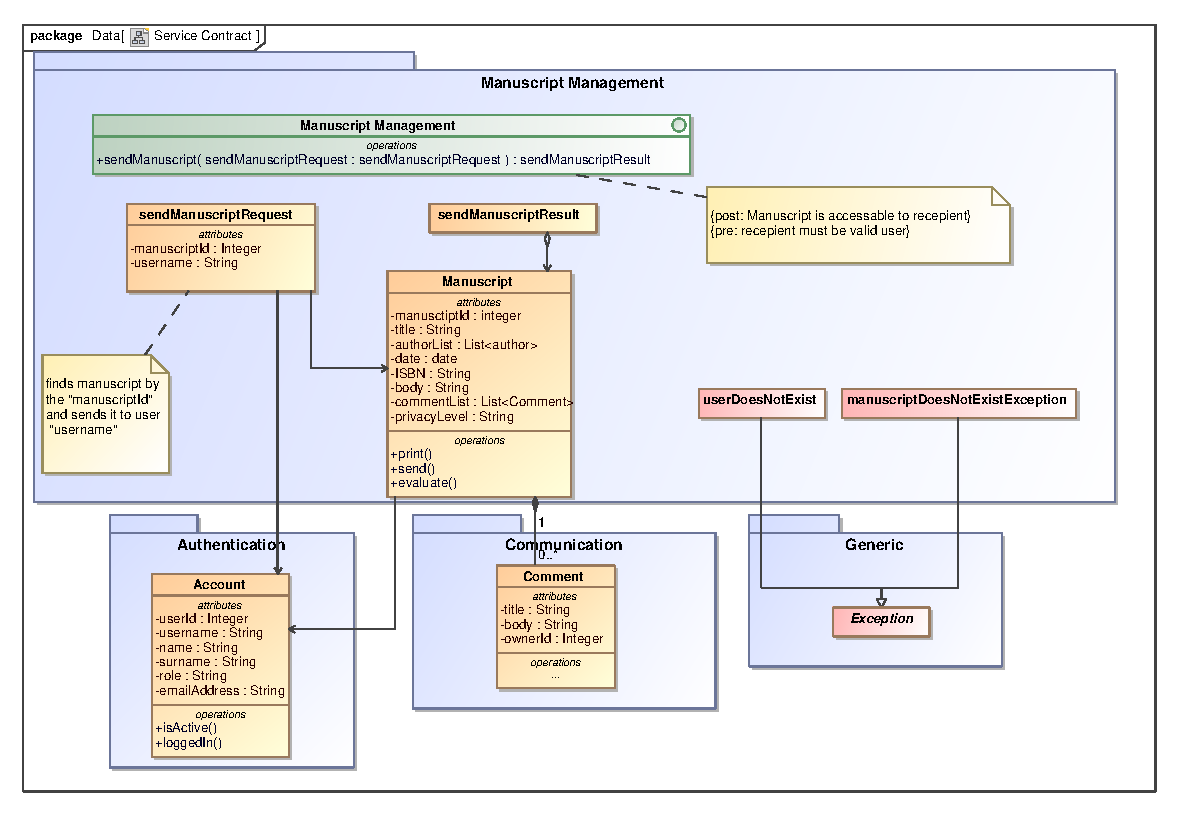
\includegraphics[height=330px, width=500px]{epsImages/ManuscriptManagement/sendManuscriptServiceContract.eps}
\caption{Service contract for sending a manuscript}
\end{figure}
 \newpage
\subsubsection{Domain Model} 
\par {This module will keep a manuscript in the database as well as be connected to all the other modules needed to perform the necessary tasks such as communication, adding authors,editors,agents etc, the modules connected to this module at the current stage of management are: Communication, Authentication as well as the external classes required for linking the manuscript to social media.}

 \begin{figure}[h]
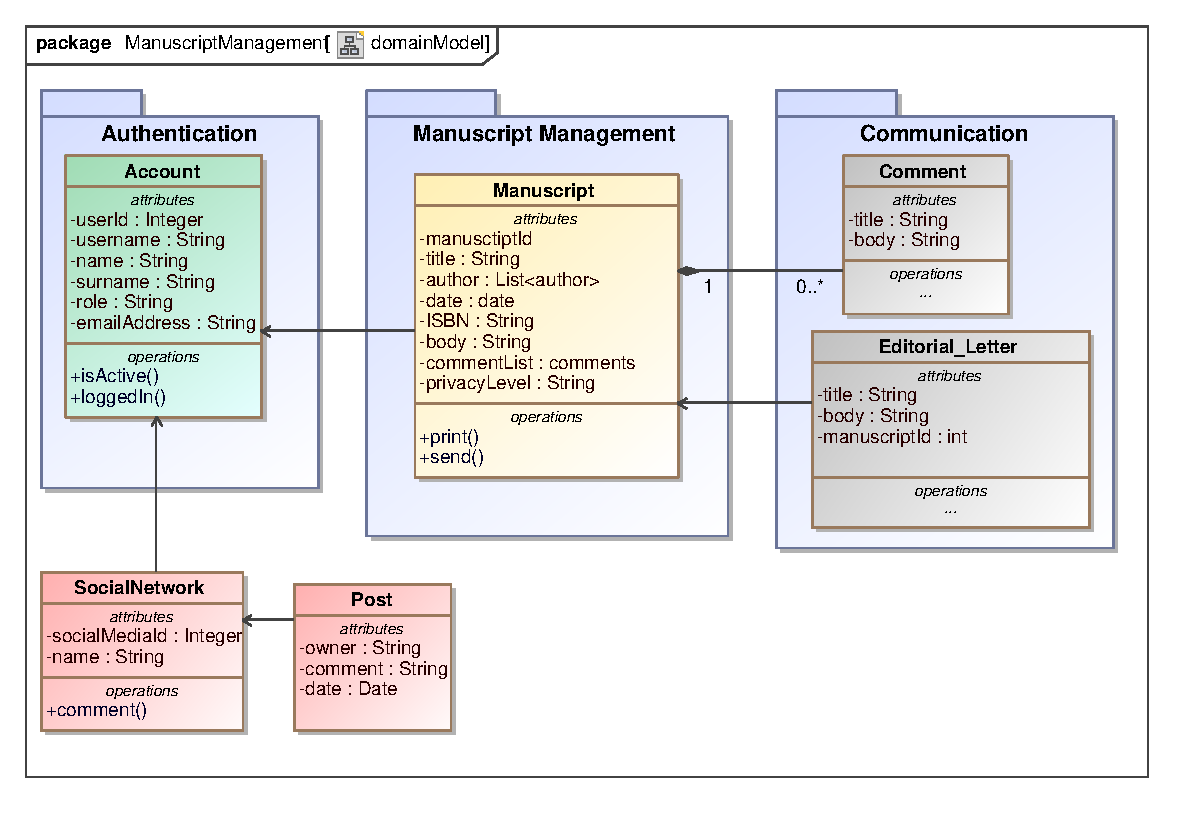
\includegraphics[height=350px, width=500px]{epsImages/DomainModels/ManuscriptManagement.eps}
\caption{Domain model for managing a manuscript}
\end{figure}

\end{enumerate}

\newpage

\subsection{Reporting}

\subsubsection{scope}
\par{This section provides the details use case requirements for the use cases offered by the Authentication
module.}

\begin{figure}[h]
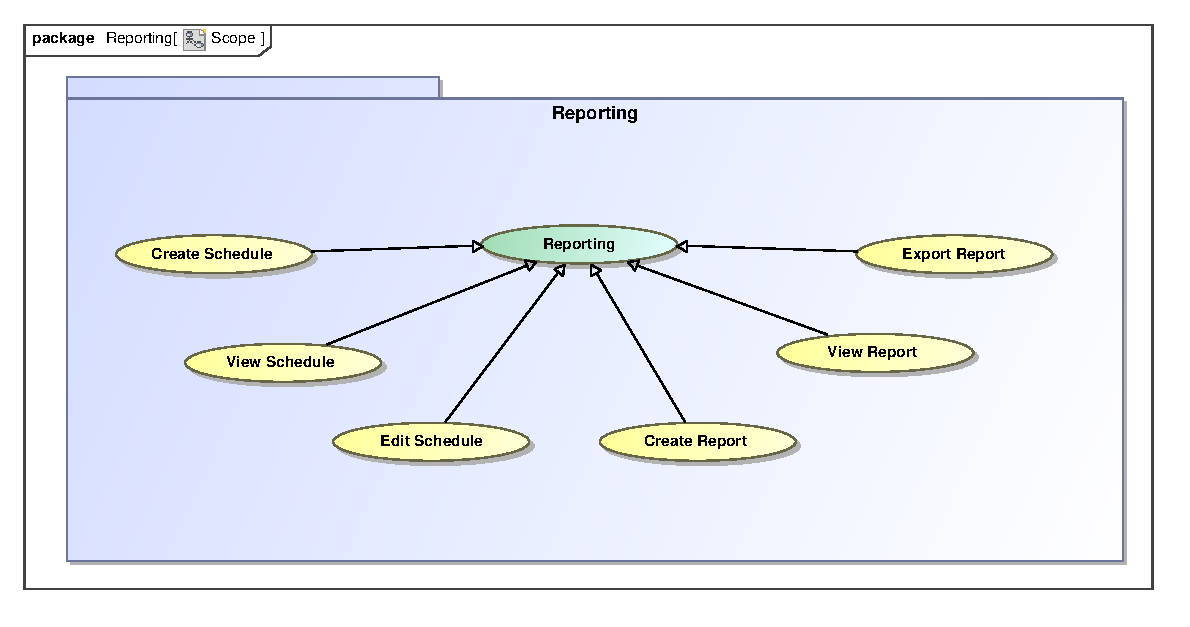
\includegraphics[height=250px, width=500px]{epsImages/Reporting/ReportScope.eps}
\caption{Scope of Reporting module}
\end{figure}


\subsubsection{Use Cases}

\begin{enumerate}
\item \textbf{CreateSchedule - priority: important}
\par{This use case allows a user to create a work schedule for the book that may consist of multiple tasks.}

\begin{figure}[h]
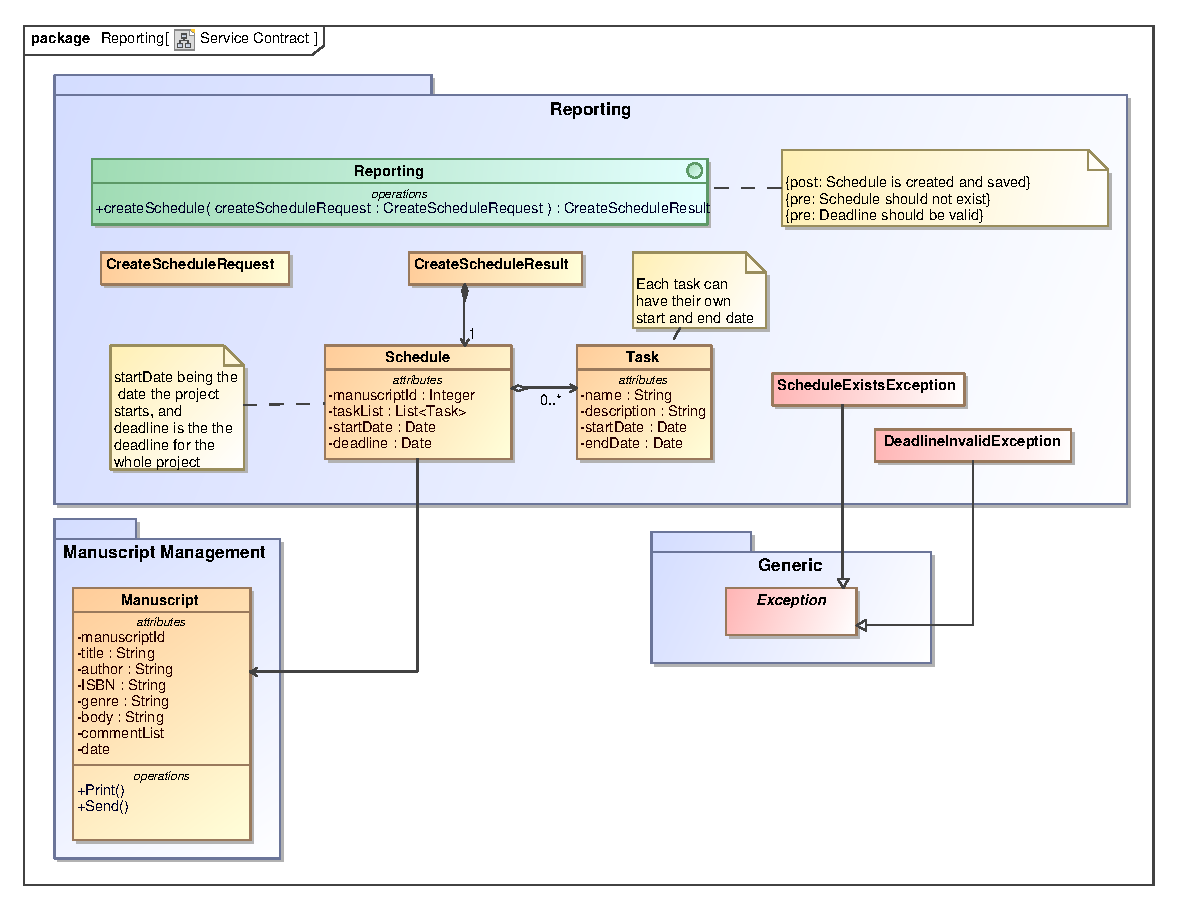
\includegraphics[height=250px, width=500px]{epsImages/Reporting/createSchedule.eps}
\caption{Service contract for creating a work schedule}
\end{figure}

\item \textbf{ViewSchedule - priority: important}
\par{This use case allows a user to view the work schedule for the book.}

\begin{figure}[h]
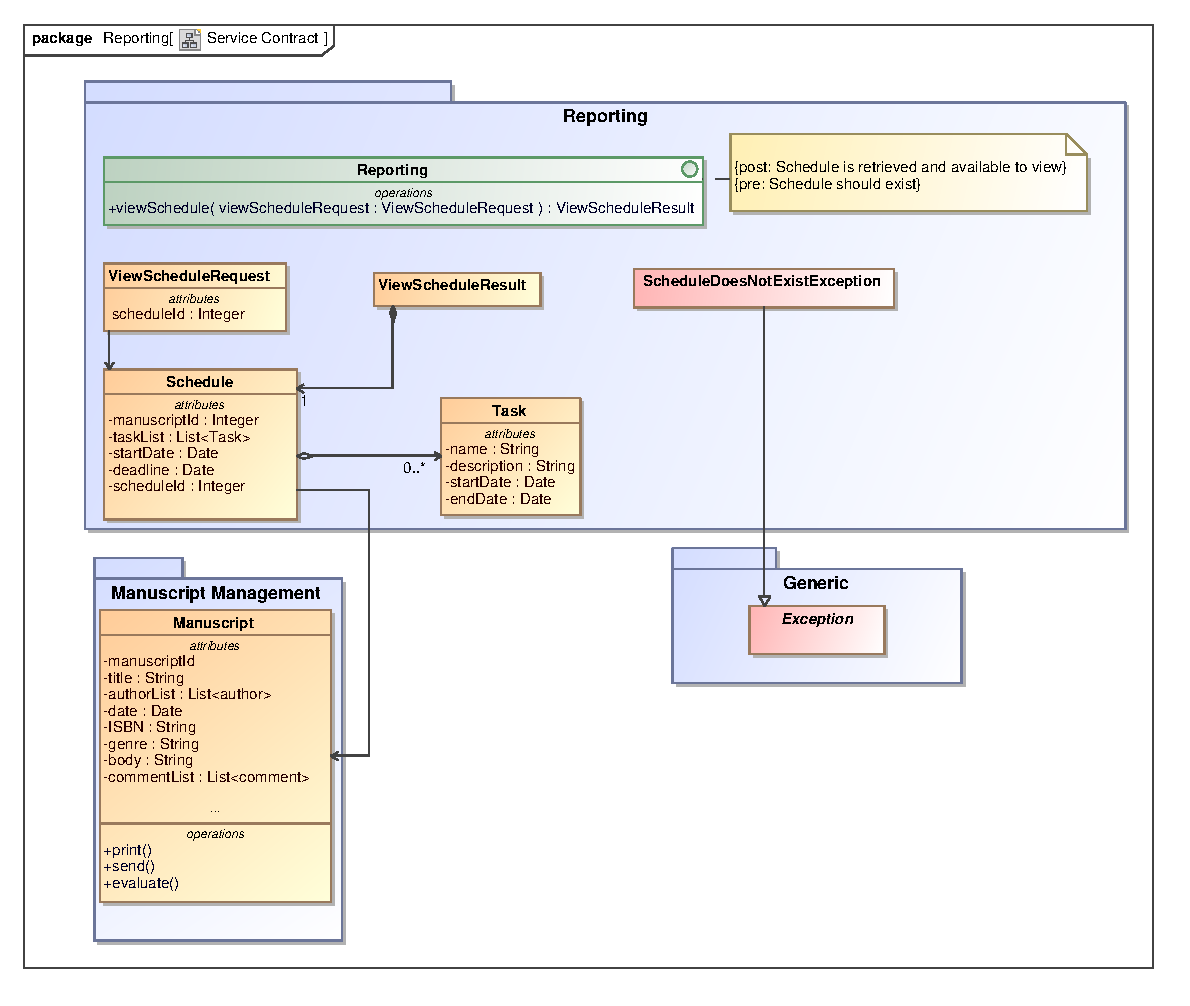
\includegraphics[height=250px, width=500px]{epsImages/Reporting/viewSchedule.eps}
\caption{Service contract for viewing a work schedule}
\end{figure}

\item \textbf{EditSchedule - priority: important}\\
\par{This use case allows a user to make changes to the work schedule of the book.}
\par{\textbf{service contract:} below is the service contract for editing a work schedule}

\begin{figure}[h]
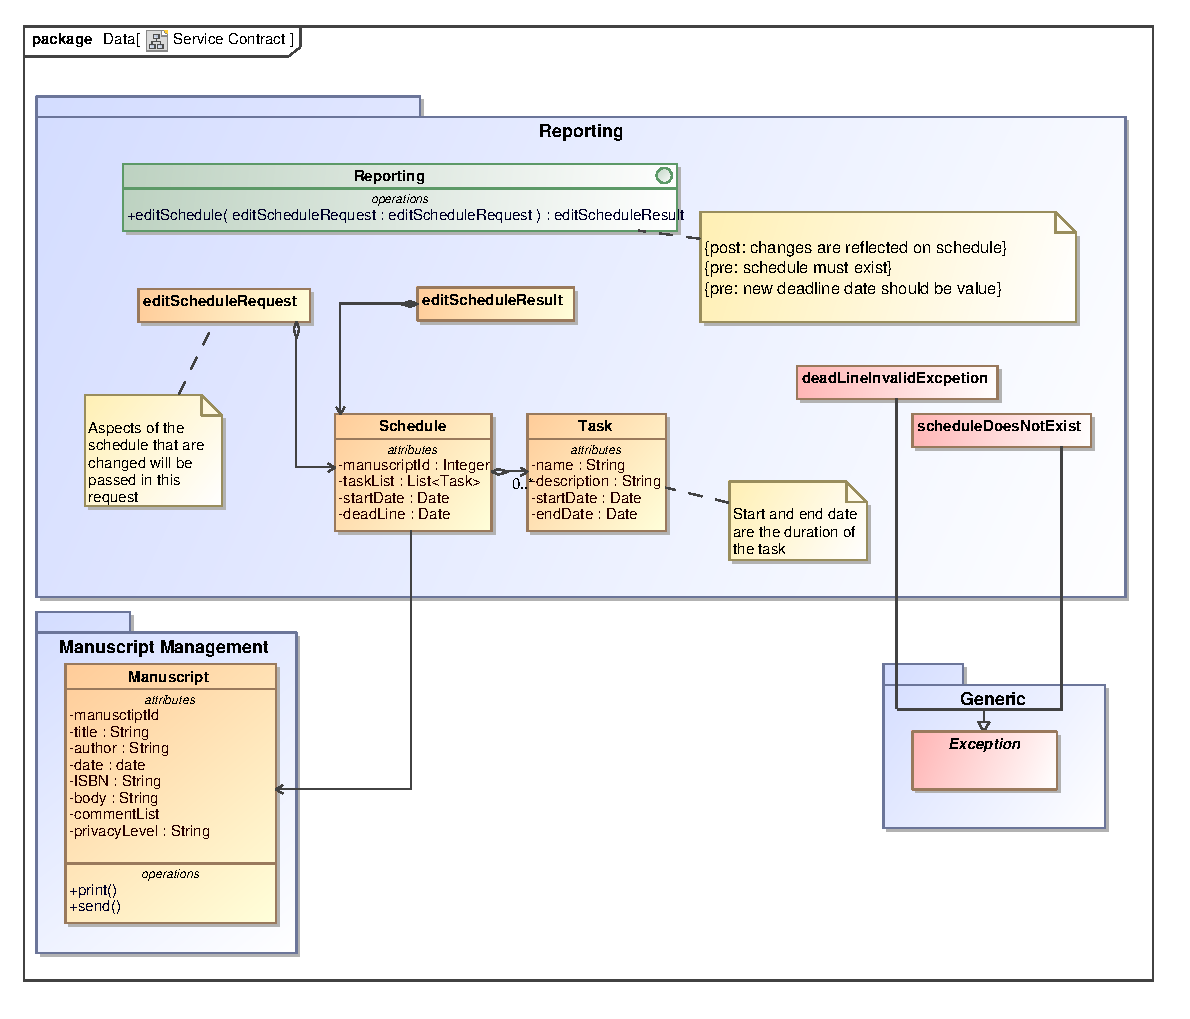
\includegraphics[height=250px, width=500px]{epsImages/Reporting/editScheduleServiceContract.eps}
\caption{Service contract for editing a work schedule}
\end{figure}

\item \textbf{createReport - priority: important}\\
\par{This use case creates  a report based on filters and provides it in printable format.}\\
\par{\textbf{service contract:} The service contract for the createReport  service is shown in figure below. The pre-conditions are enforced (raising the appropriate exception should they not be met) and the report is created and return in a printable format.}

\begin{figure}[h]
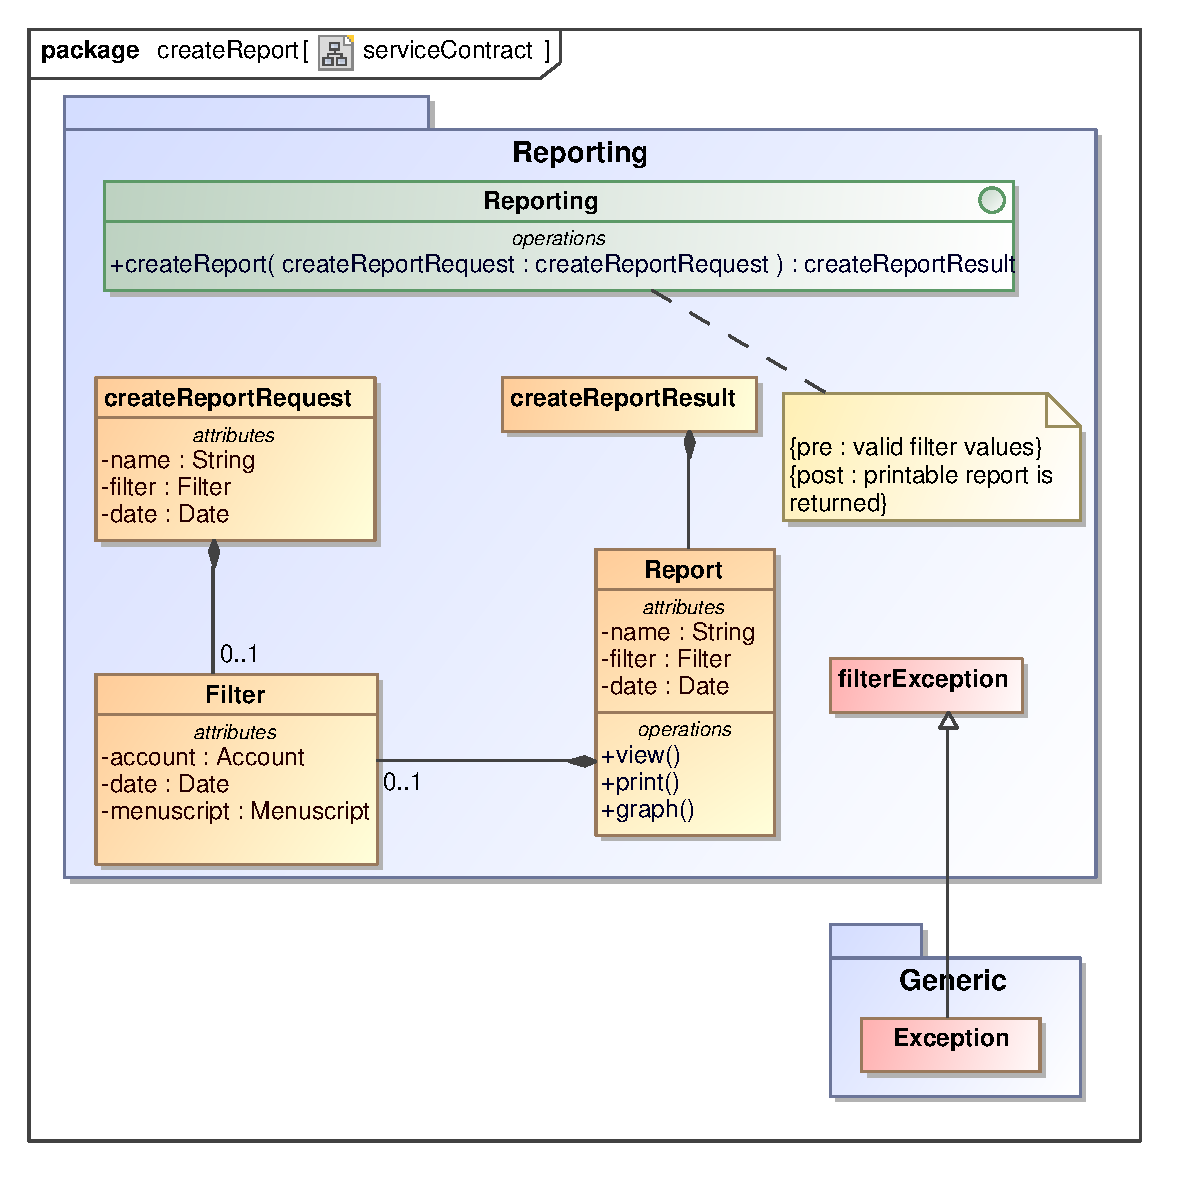
\includegraphics[height=250px, width=500px]{epsImages/Reporting/createReport.eps}
\caption{Service contract for creating a report}
\end{figure}

\item \textbf{viewReport - priority: important}\\
\par{This use case allows users to view a generated report, on the system (before exporting to say, a pdf for example).}\\
\par{\textbf{service contract:} Below is the service contract for viewing a report.}

\begin{figure}[h]
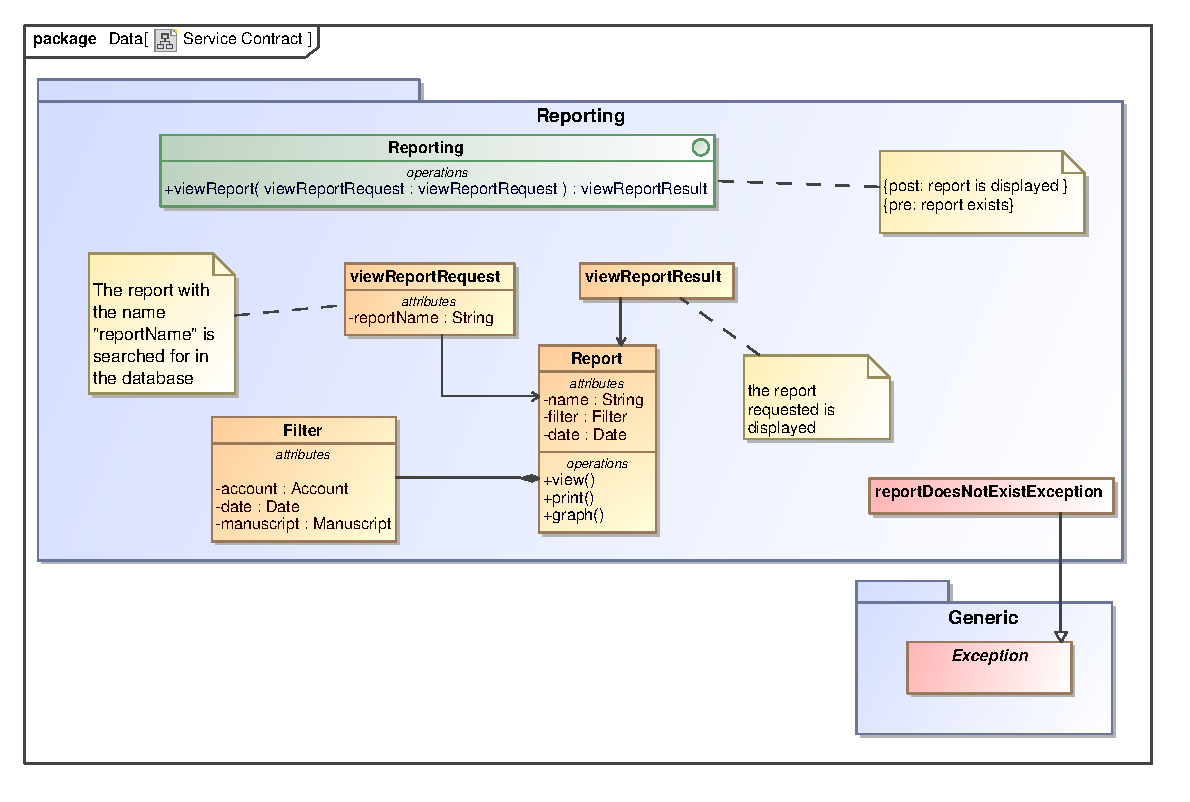
\includegraphics[height=250px, width=500px]{epsImages/Reporting/viewReportServiceContract.eps}
\caption{Service contract for viewing a report}
\end{figure}

 
\item \textbf{exportReport}
\par{priority: important  This use case which allows one to export a manuscript}\\
\par{\textbf{service contract:}} 

\begin{figure}[h]
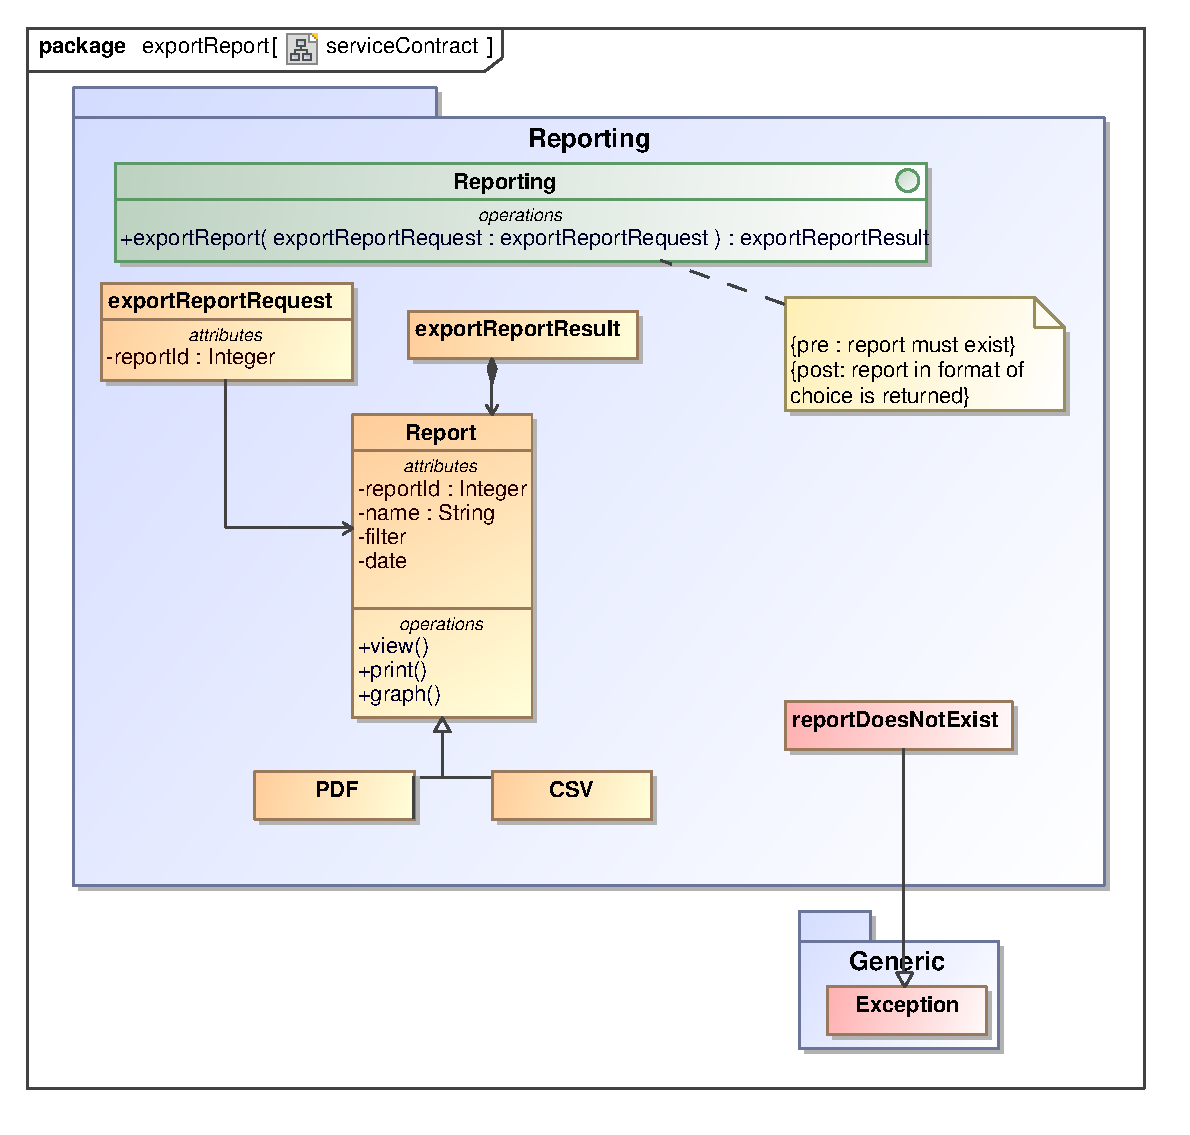
\includegraphics[height=250px, width=500px]{epsImages/Reporting/exportReport.eps}
\caption{Service contract for exporting a report}
\end{figure}
\end{enumerate}

\newpage

\clearpage
\subsection{Communication}

\subsubsection{scope}
\par{In the life cycle of the book, there is plenty communication that occurs. This module takes care of all communication that may occur between different parties (author to editor, editor to agent agent to author etc)}

\begin{figure}[h]
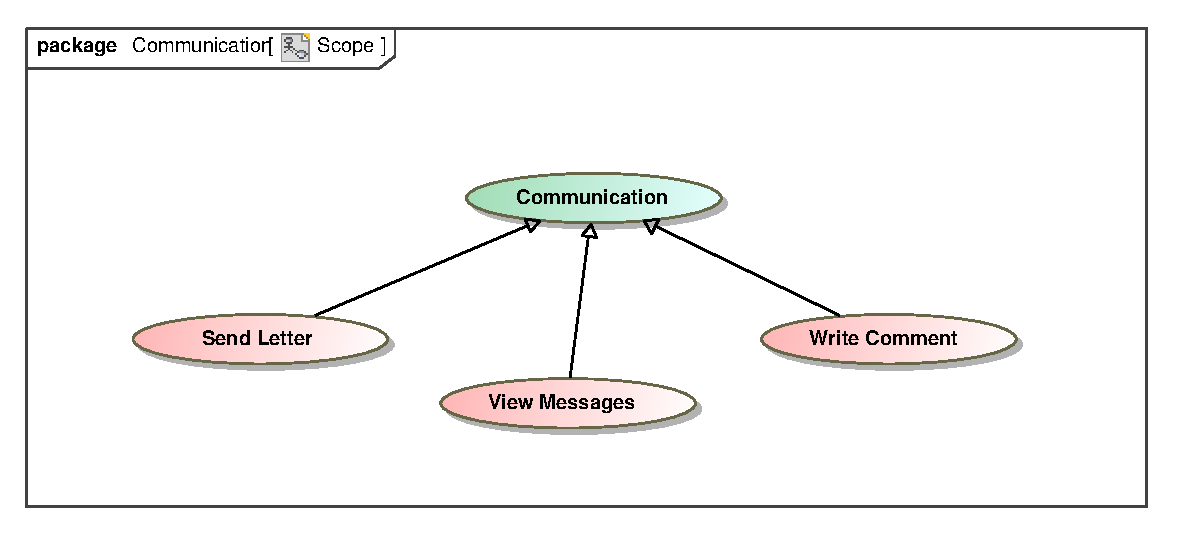
\includegraphics[scale=0.9]{epsImages/Communication/CommunicationScope.eps}
\caption{Scope of Communication module}
\end{figure}

\newpage
\subsubsection{Use Cases}

\begin{enumerate}
\item \textbf{Send Letter - priority: critical}
\par{This use case allows the writing and sending of an appropriate letter/message to the corresponding user, such as a query letter from author to agent. Available letters are: editorial letter, contract offer and query letter}

\begin{figure}[h]
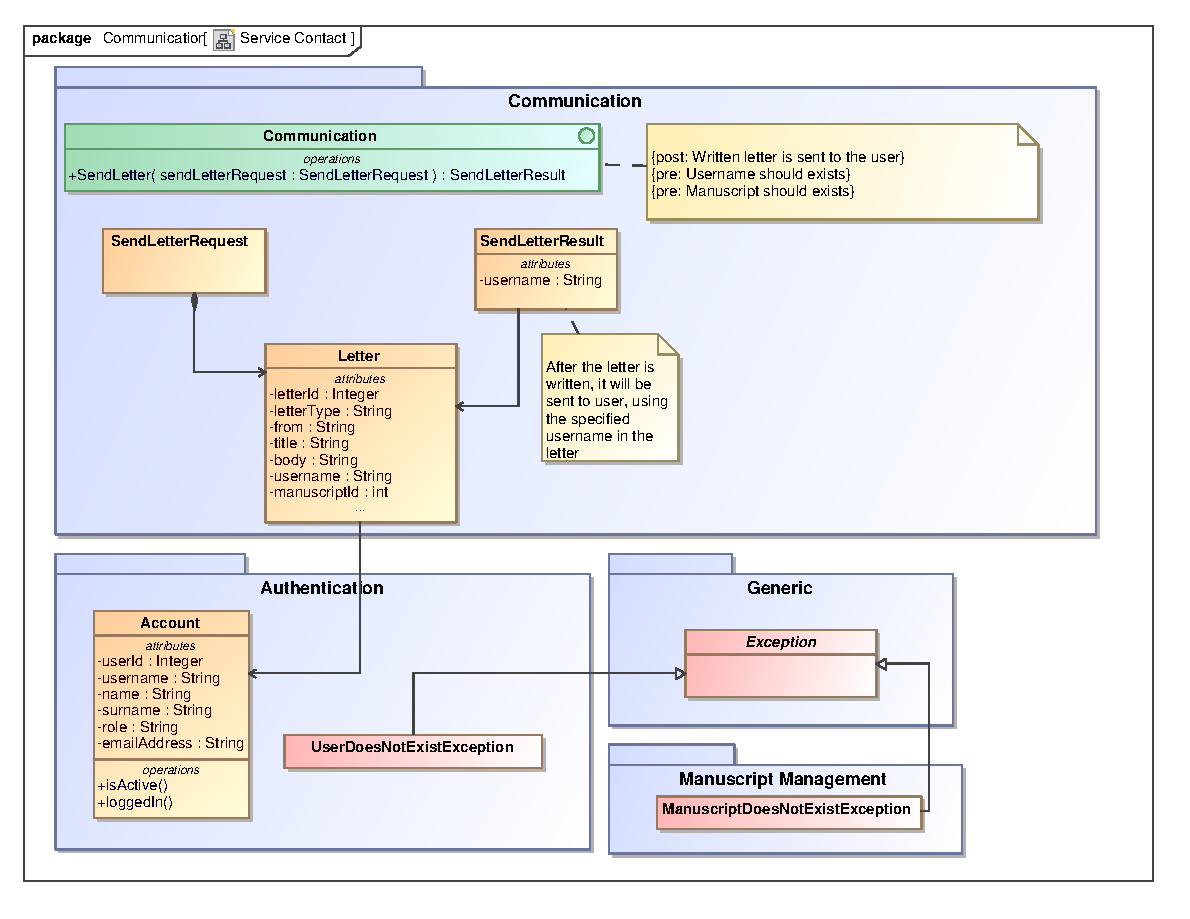
\includegraphics[scale=0.9]{epsImages/Communication/sendLetterServiceContract.eps}
\caption{Service contract for sending a letter}
\end{figure}

\newpage
\item \textbf{View Letter - priority: critical}\\
\par{This use case allows a user to view one of the letters sent to him/her. The letter can be an editorial letter, contract offer or query letter }\\ \\

\textbf{service contract:}

\begin{figure}[h]
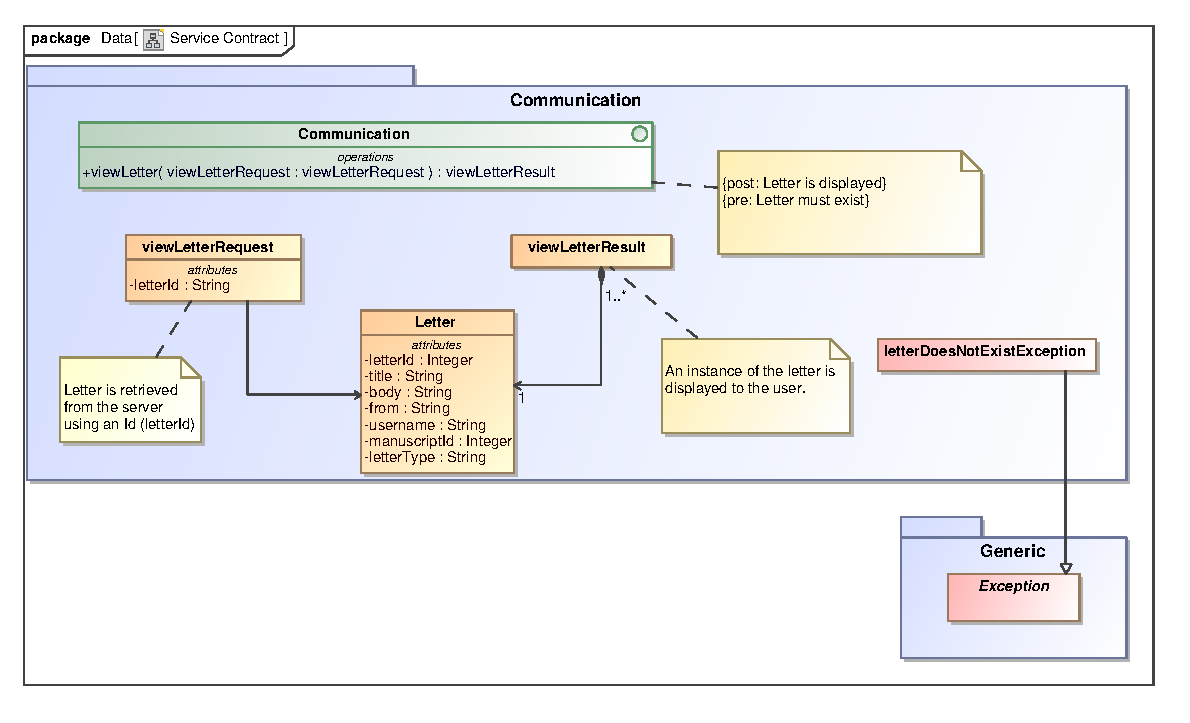
\includegraphics[scale=0.9]{epsImages/Communication/viewLetterServiceContract.eps}
\caption{Service contract for viewing a letter}
\end{figure}

\newpage

\item \textbf{Write Comment priority: nice to have}\\
\par{This allows a user (with the editor role) to add comments on the manuscript. Comments can be little notes to the author to indicate what the editor was thinking about that portion of the manuscript.}

\begin{figure}[h]
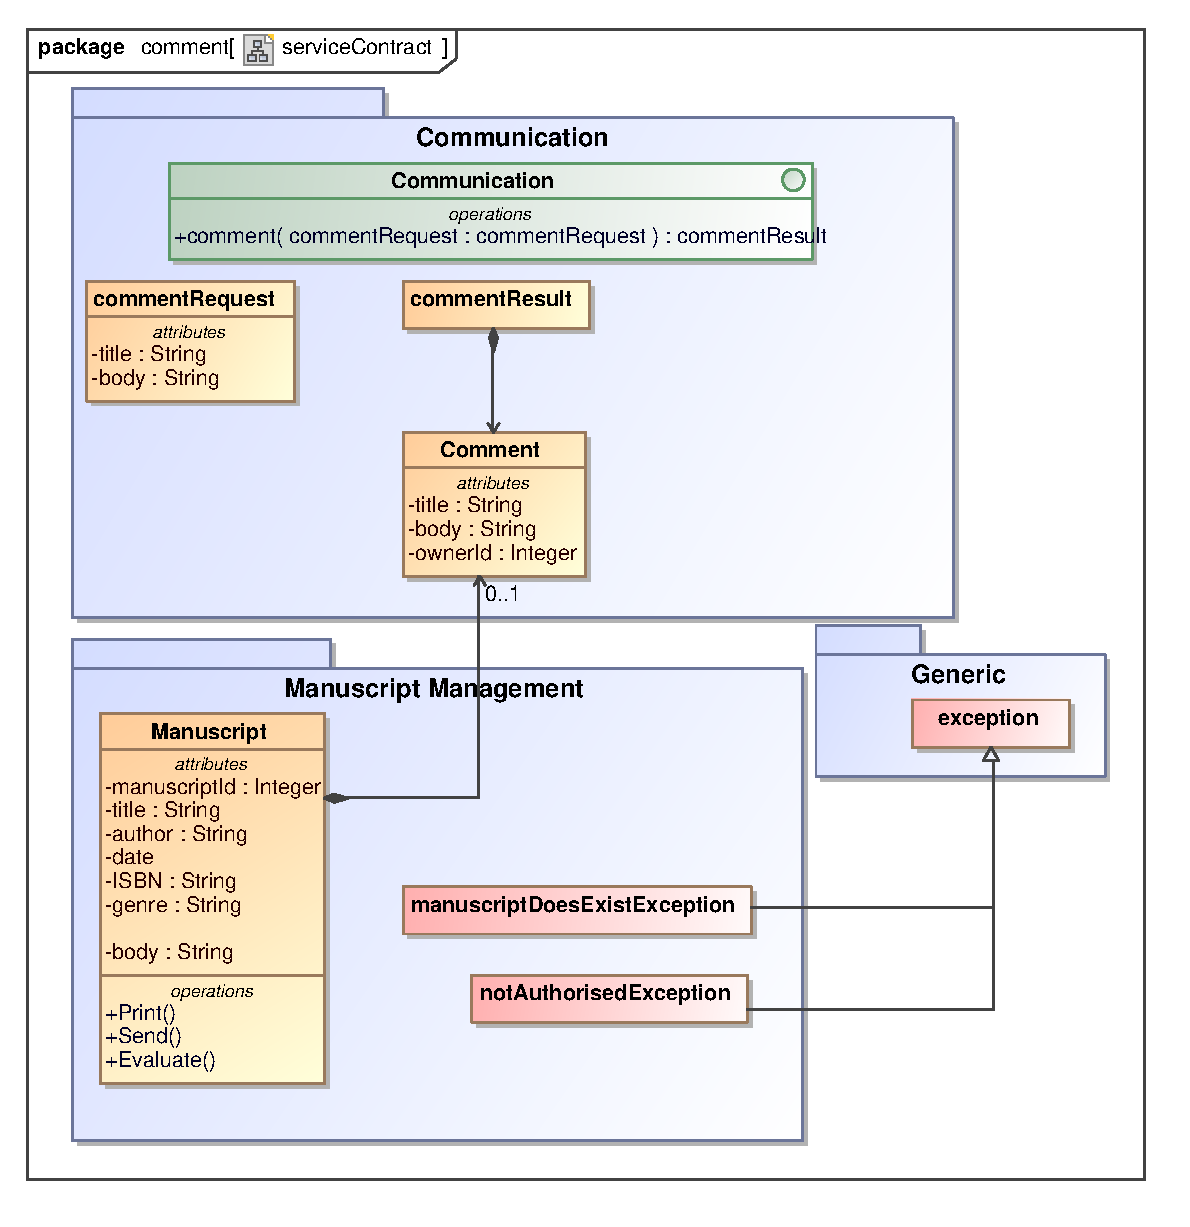
\includegraphics[scale=0.8]{epsImages/Communication/comment.eps}
\caption{Service contract for writing a comment a manuscript}
\end{figure}

\end{enumerate}

\subsubsection{Domain Model}
\par{Every time a user wishes to communicate with another user on the system they will make use of functionality from this module. This module accommodates the sending, receiving and viewing of any messages on the system between users.}

\begin{figure}[h]
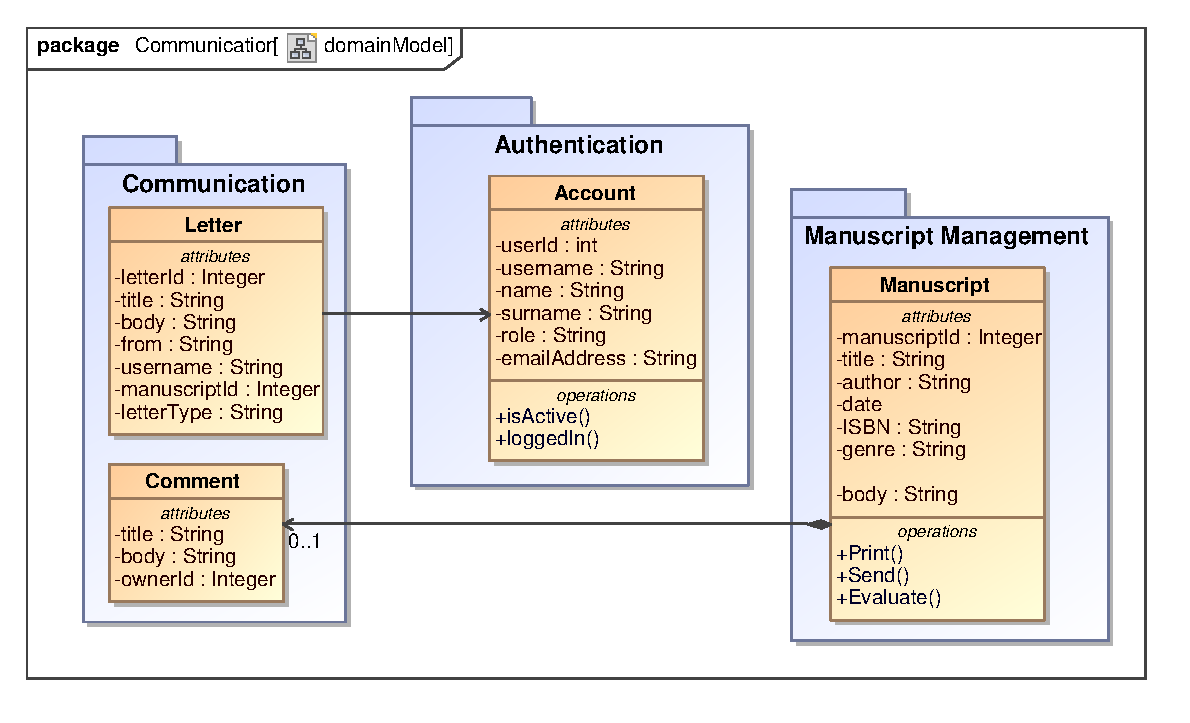
\includegraphics[scale=0.8]{epsImages/DomainModels/communicationDomainModel.eps}
\caption{Service contract for writing a comment a manuscript}
\end{figure}
\newpage

\clearpage
\subsection{Design}

\subsubsection{scope}
\par{The design module allows the designer/design team to structure the layout of the book.This is done by creating or choosing a template, as well as uploading all desired graphics and designing the books cover pages.}

\begin{figure}[h]
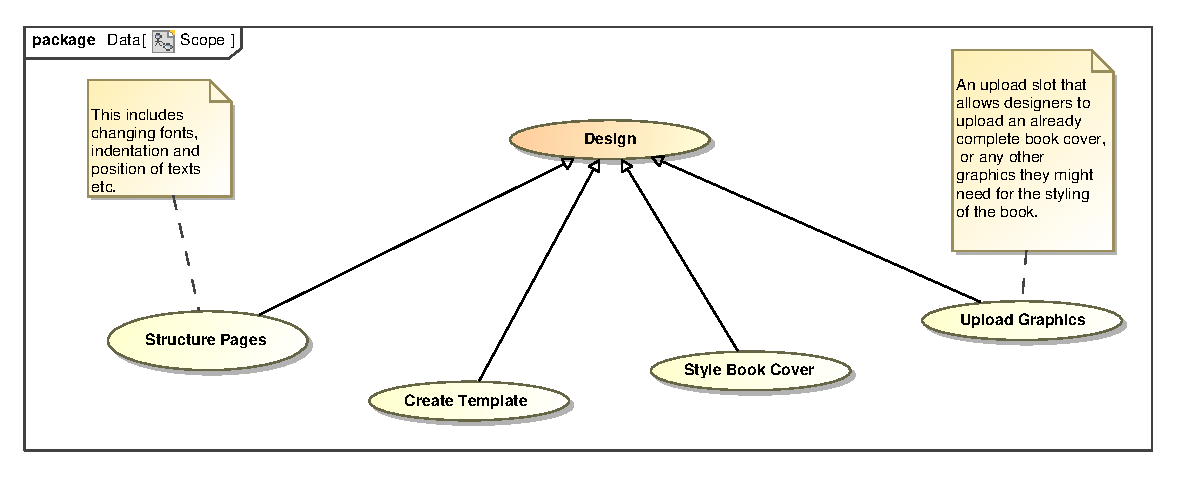
\includegraphics[scale=0.9,width=450px]{epsImages/Design/Scope.eps}
\centering
\caption{Scope of Design module}
\end{figure}

\newpage
\subsubsection{Use Cases}
\begin{enumerate}
\item \textbf{Structure Pages - priority: critical}
\par{This use case which allows one to structure the  manuscript.}
\par{\textbf{Service Contract:}
}
\begin{figure}[h]
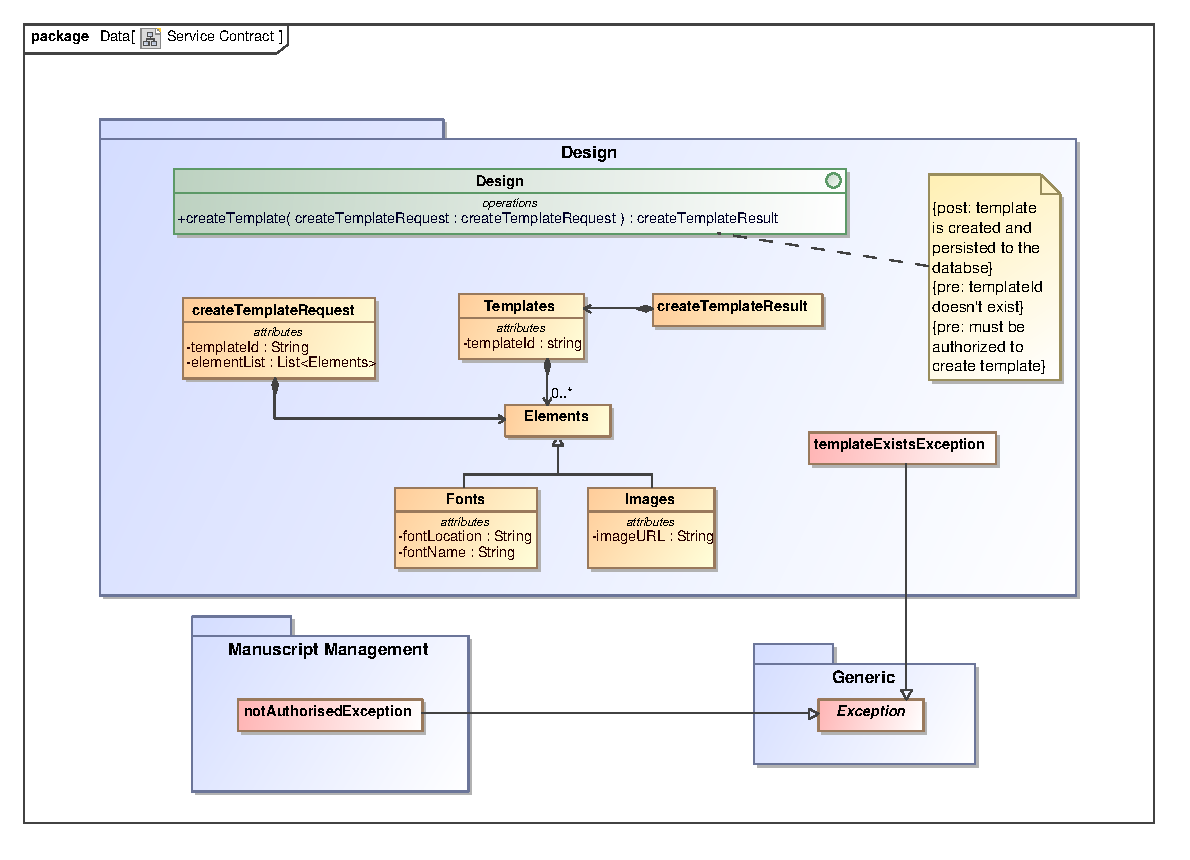
\includegraphics[scale=0.8,width=400px]{epsImages/Design/createTemplateServiceContract.eps}
\centering
\caption{Service contract for structuring a menuscript}
\end{figure}

\newpage
\item \textbf{Create Template - priority: nice to have}
\par{This module allows a user to create a template design for the book.}
\par{\textbf{Service Contract:} 
}
 \begin{figure}[h]
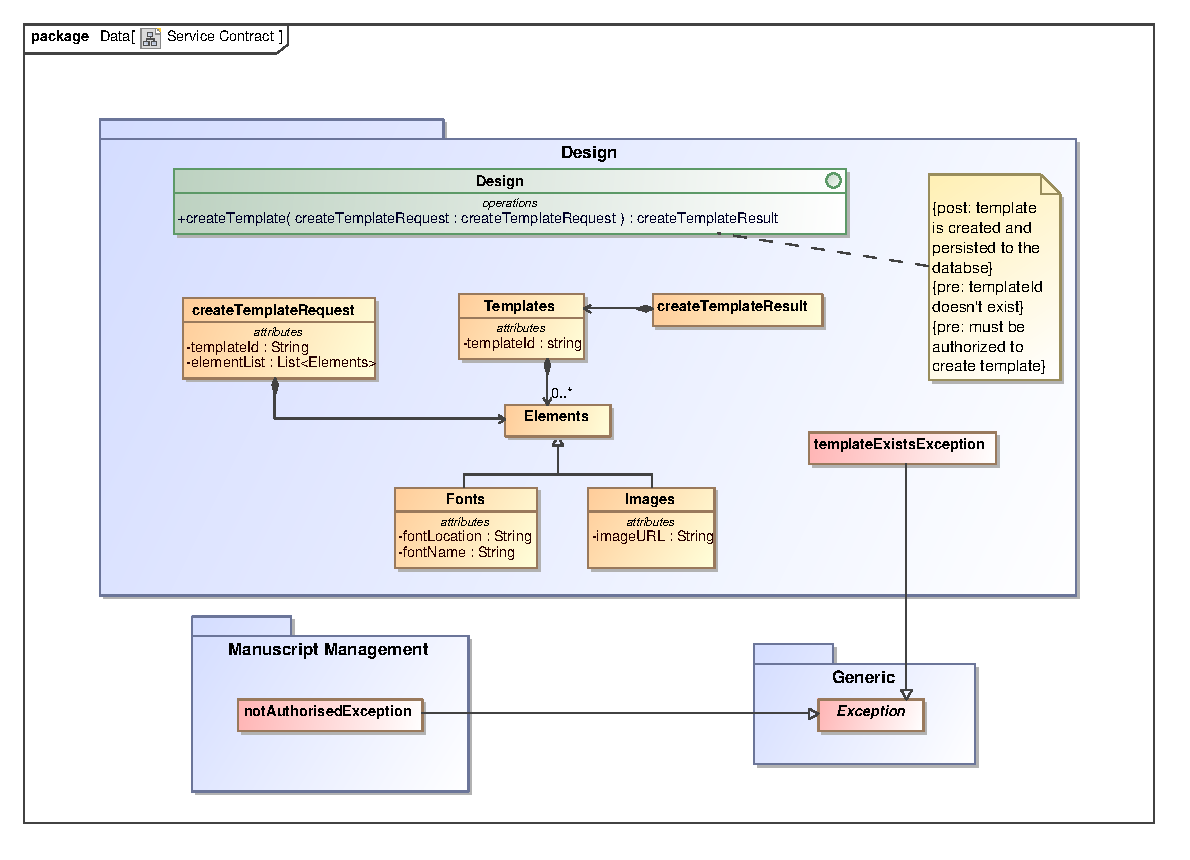
\includegraphics[scale=0.8,width=400px]{epsImages/Design/createTemplateServiceContract.eps}
\centering
\caption{Service contract for creating a template design}
\end{figure}

\newpage
\item \textbf{Create Book Cover - priority: critical}
\par{This use case which allows create a book cover for a  manuscript.}
\par{\textbf{Service Contract:} 
}
 \begin{figure}[h]
\centering
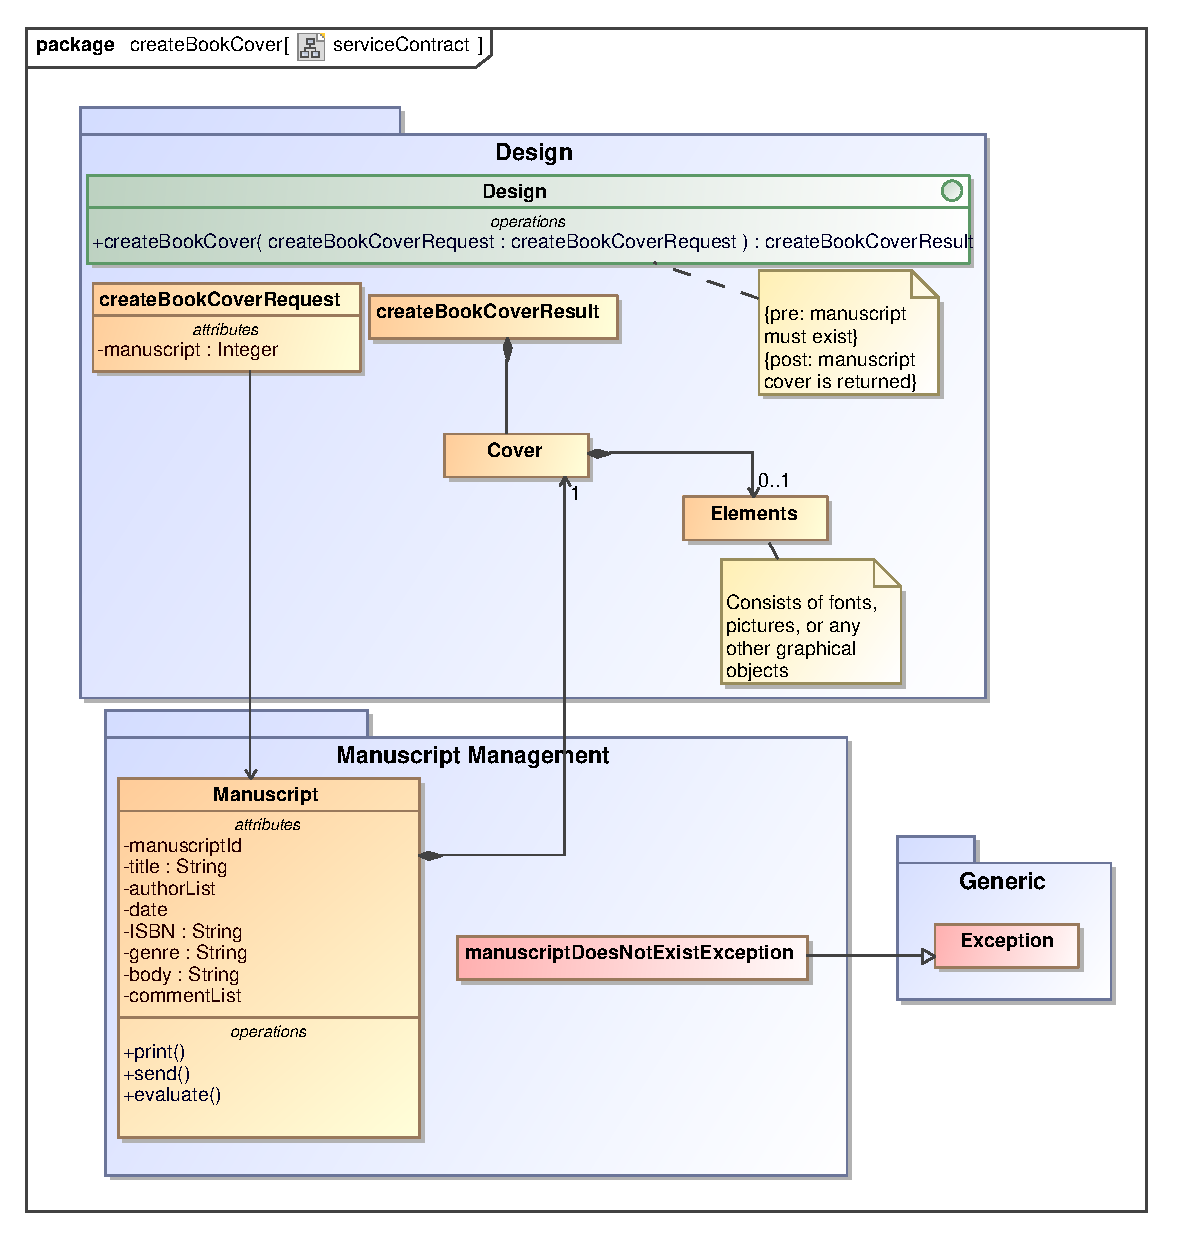
\includegraphics[scale=0.8,width=400px]{epsImages/Design/createBookCover.eps}
\caption{Service contract for creating a book cover}
\end{figure}

\newpage
\item \textbf{Upload Graphic - priority: important}\\
\par{This use case allows a user to open any graphic they choose. This may be a new font, or image they wish to use, or a completed cover for the book. Size and format of a graphic are restricted however.}
\par{\textbf{Service Contract:}}
\begin{figure}[h]
\centering
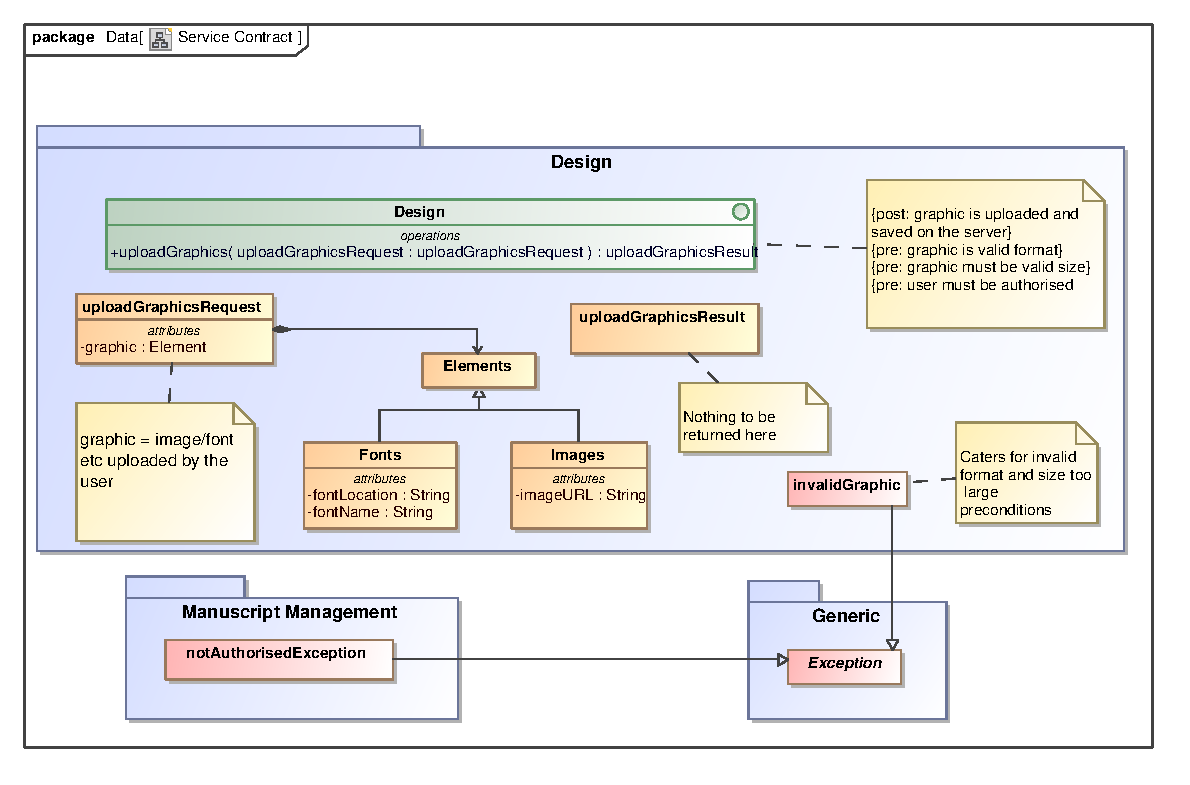
\includegraphics[scale=0.8,width=400px]{epsImages/Design/uploadGraphicsServiceContract.eps}
\caption{Service contract for uploading a graphic}
\end{figure}
\end{enumerate}

\newpage
\subsubsection{Domain Model}
\par{The design elements of the designers role is accommodated in this package. It works with elements of the Manuscript Management package as it manipulates the manuscript. }

\begin{figure}[h]
\centering
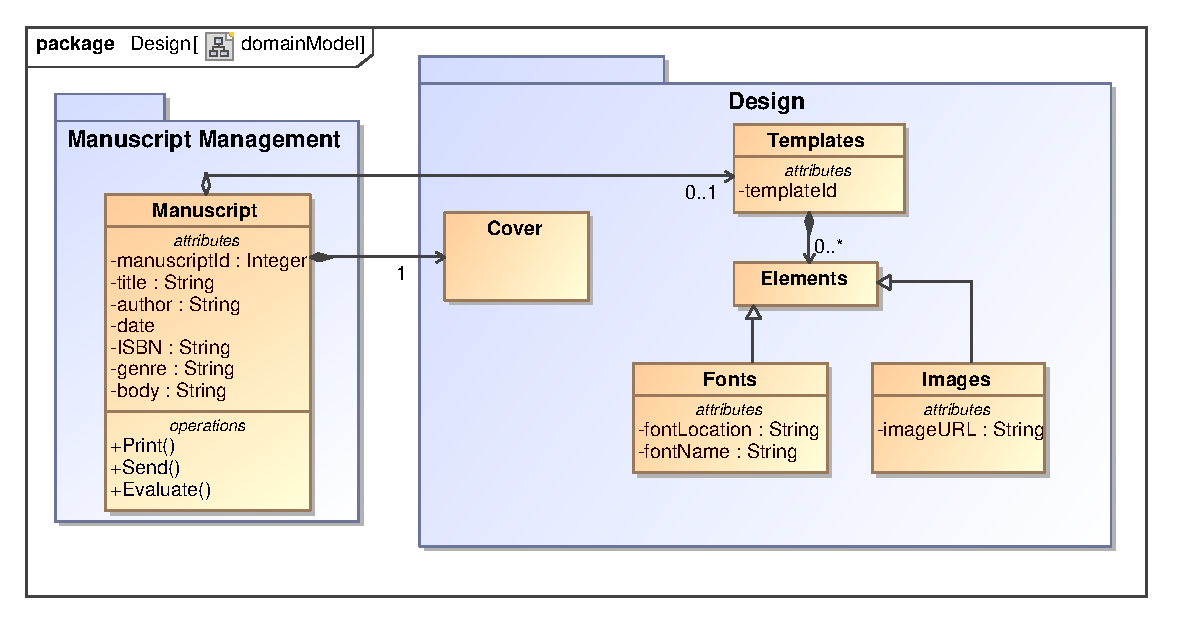
\includegraphics[scale=0.8,width=400px]{epsImages/DomainModels/DesignDomainModel.eps}
\caption{Design module's Domain Model}
\end{figure}

\newpage

\clearpage
\subsection{Production}

\subsubsection{scope}
\par{This section provides the detailed use case requirements for the use cases offered by the Production
module.}

\begin{figure}[h]
	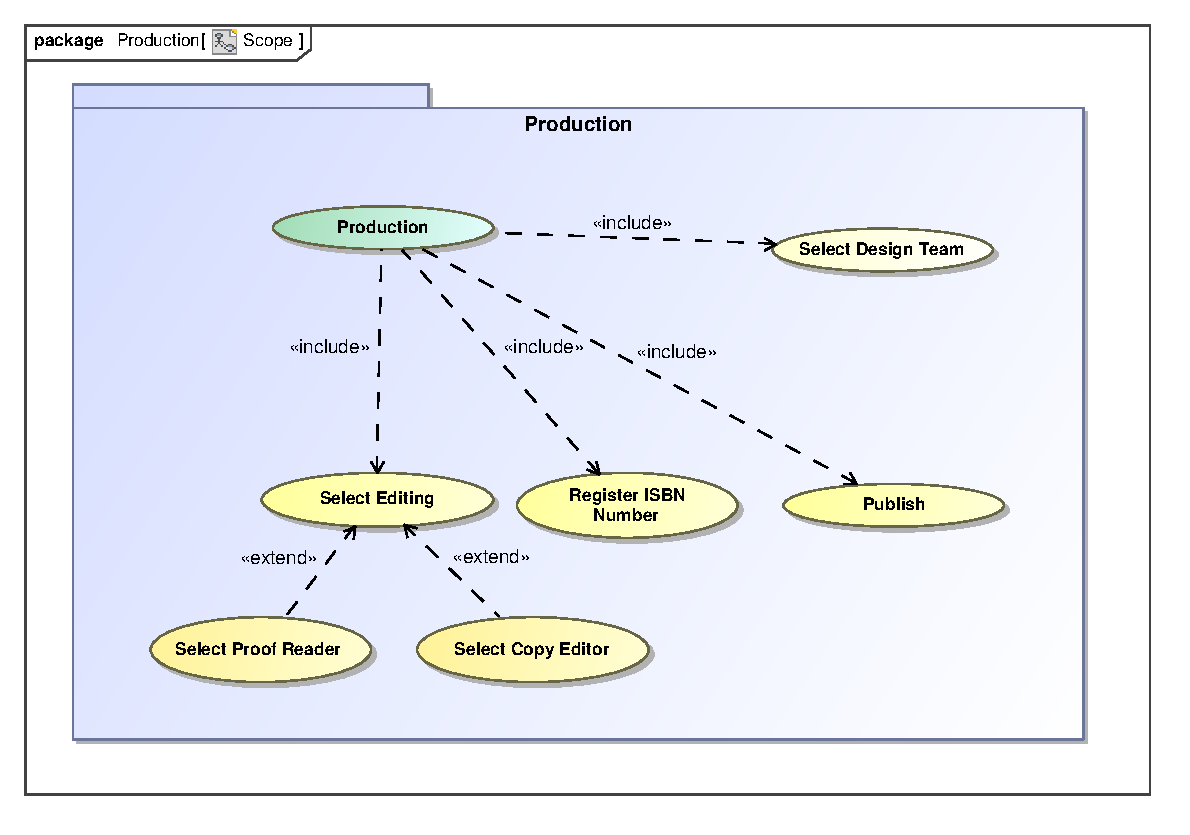
\includegraphics[height=280px, width=500px]{epsImages/Production/Scope.eps}
	\caption{Scope for Production module}
\end{figure}

\newpage
\subsubsection{Use Cases}
\begin{enumerate}
\item \textbf{Register ISBN Number - priority: important}

\par{This use case will allow the user to fill in an application form to register the ISBN number of the manuscript. Most of the inputs on this application form will be auto-completed and an email requesting the ISBN Number will be sent.}

\textbf{Service Contract:} 
Below is a figure of the registerISBNNumber service contract.

\begin{figure}[h]
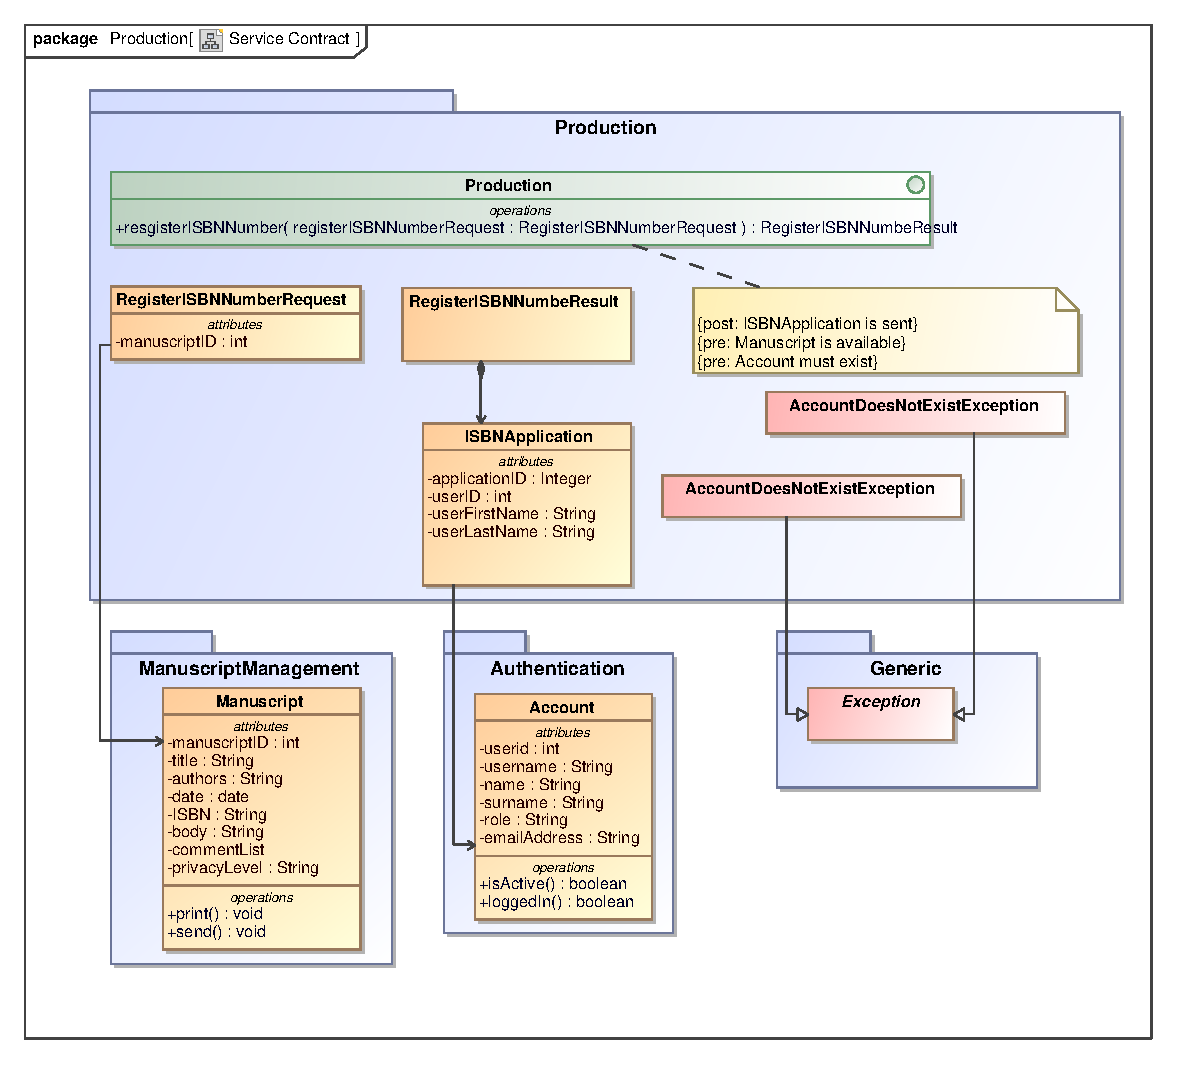
\includegraphics[height=380px, width=500px]{epsImages/Production/RegisterISBNNumber.eps}
\caption{Service contract for registering a manuscript's ISBN number.}
\end{figure}

\newpage
\item \textbf{Select Copy Editor - priority: critical}\\

\par{This use case allows a user to select a copy-editor from the available copy copy-editors registered in the system.}

\clearpage
\textbf{Service Contract:} 
The service contract for selecting a copy editor service is shown in the figure below. The pre-conditions are enforced (raising the appropriate exception should they not be met) and the required copy editor is then notified of the user's request.

\begin{figure}[h]
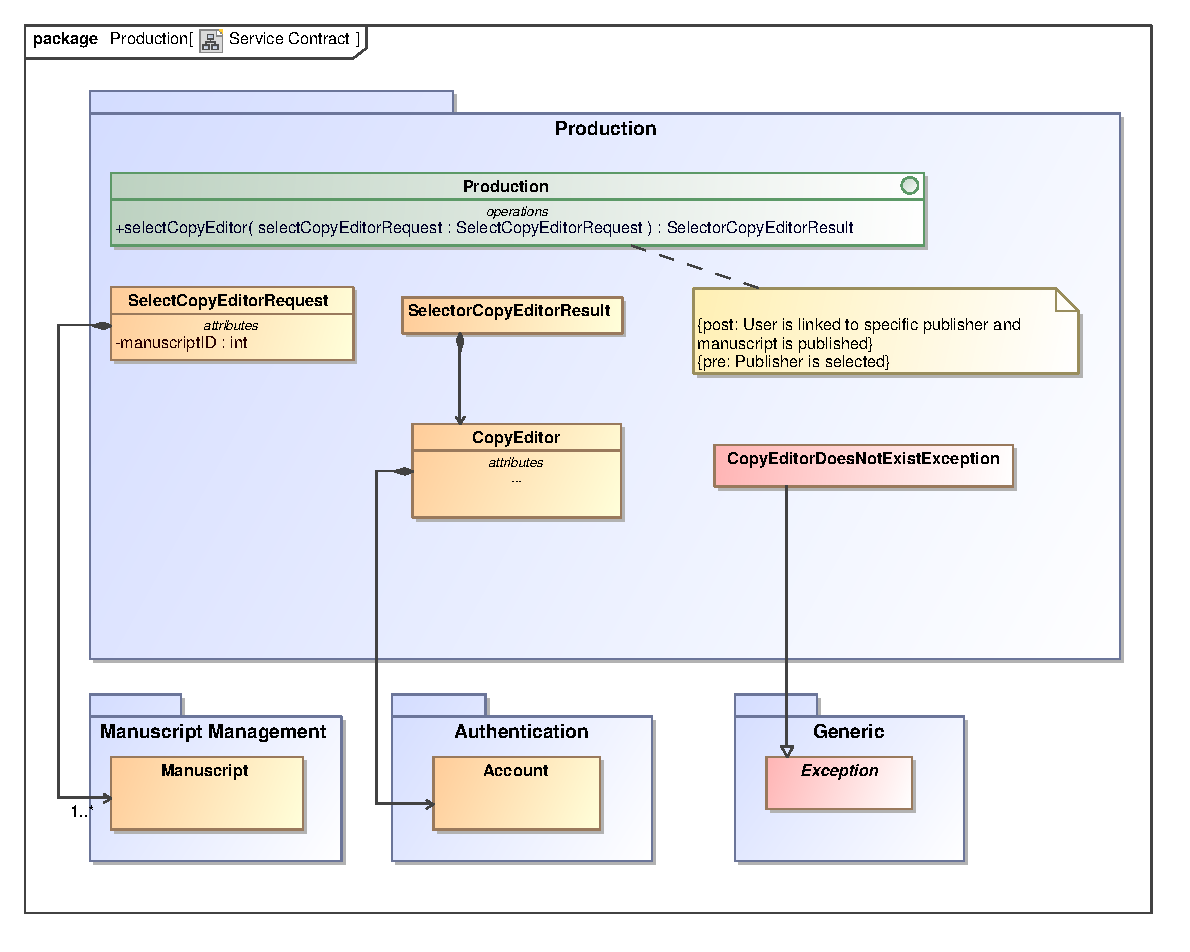
\includegraphics[height=380px, width=500px]{epsImages/Production/SelectCopyEditor.eps}
\caption{Service contract for selecting a copy editor}
\end{figure}

\newpage
\item \textbf{Select Proof Reader – priority: important}\\
\par{This use case allows a user to select a proof reader from the available proof readers registered in the system.}

\textbf{Service Contract:} 
The service contract for selecting a proof reader service is shown in the figure below. The pre-conditions are enforced (raising the appropriate exception should they not be met) and the required proof reader is then notified of the user's request.

\begin{figure}[h]
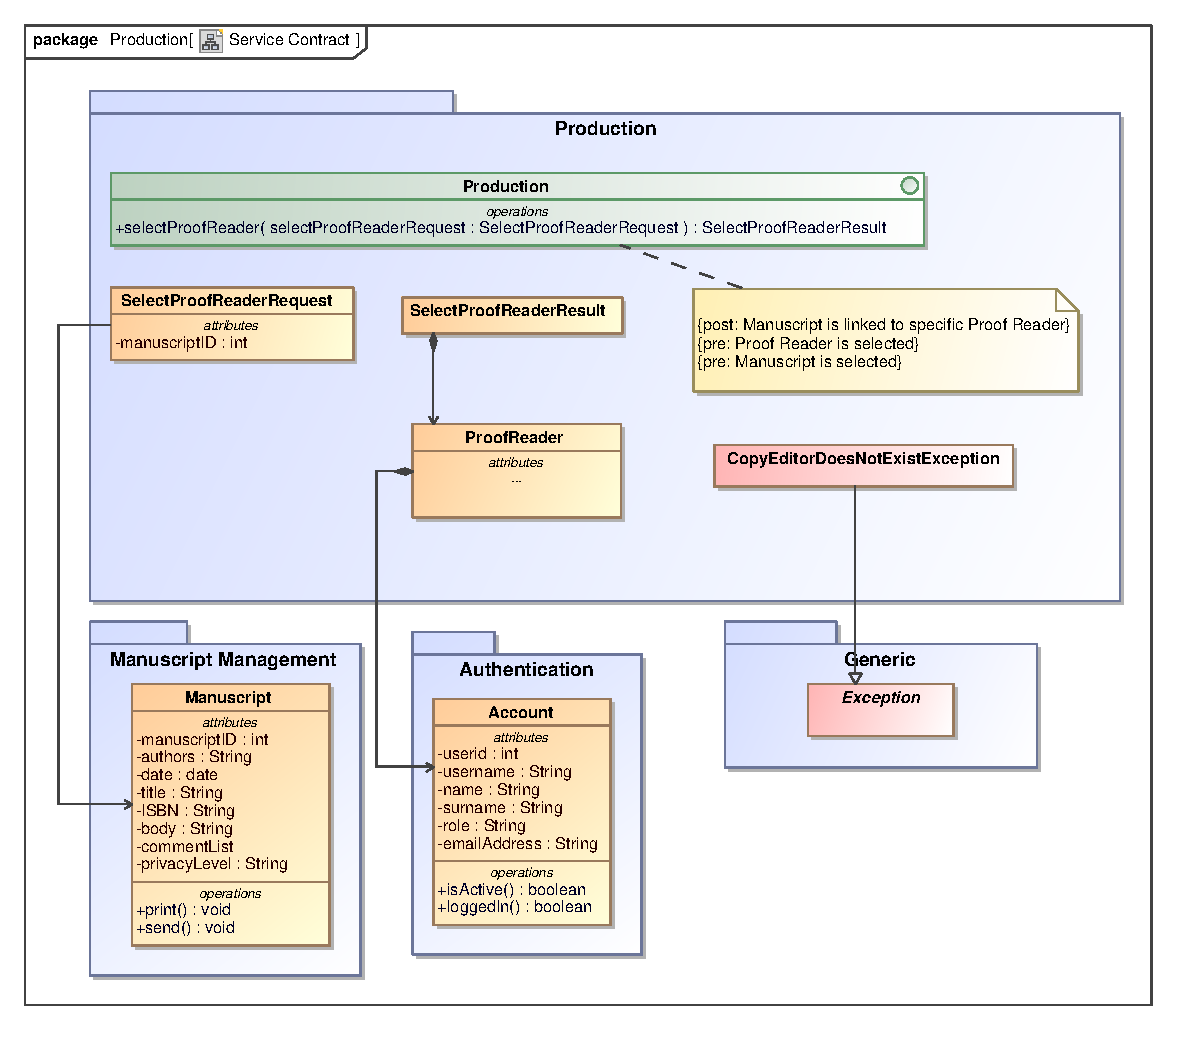
\includegraphics[height=380px, width=500px]{epsImages/Production/SelectProofReader.eps}
\caption{Service contract for selecting a proof reader}
\end{figure}

\newpage
\item \textbf{Select Design Team – priority: important}\\
\par{This use case allows a user to select, from the registered designers, a design team that will be resposible for the book cover and styling.}

\textbf{Service Contract:} 
The service contract for the selectDesignTeam service is shown in figure below. The pre-conditions are enforced (raising the appropriate exception should they not be met) and the required design team is notified.

\begin{figure}[h]
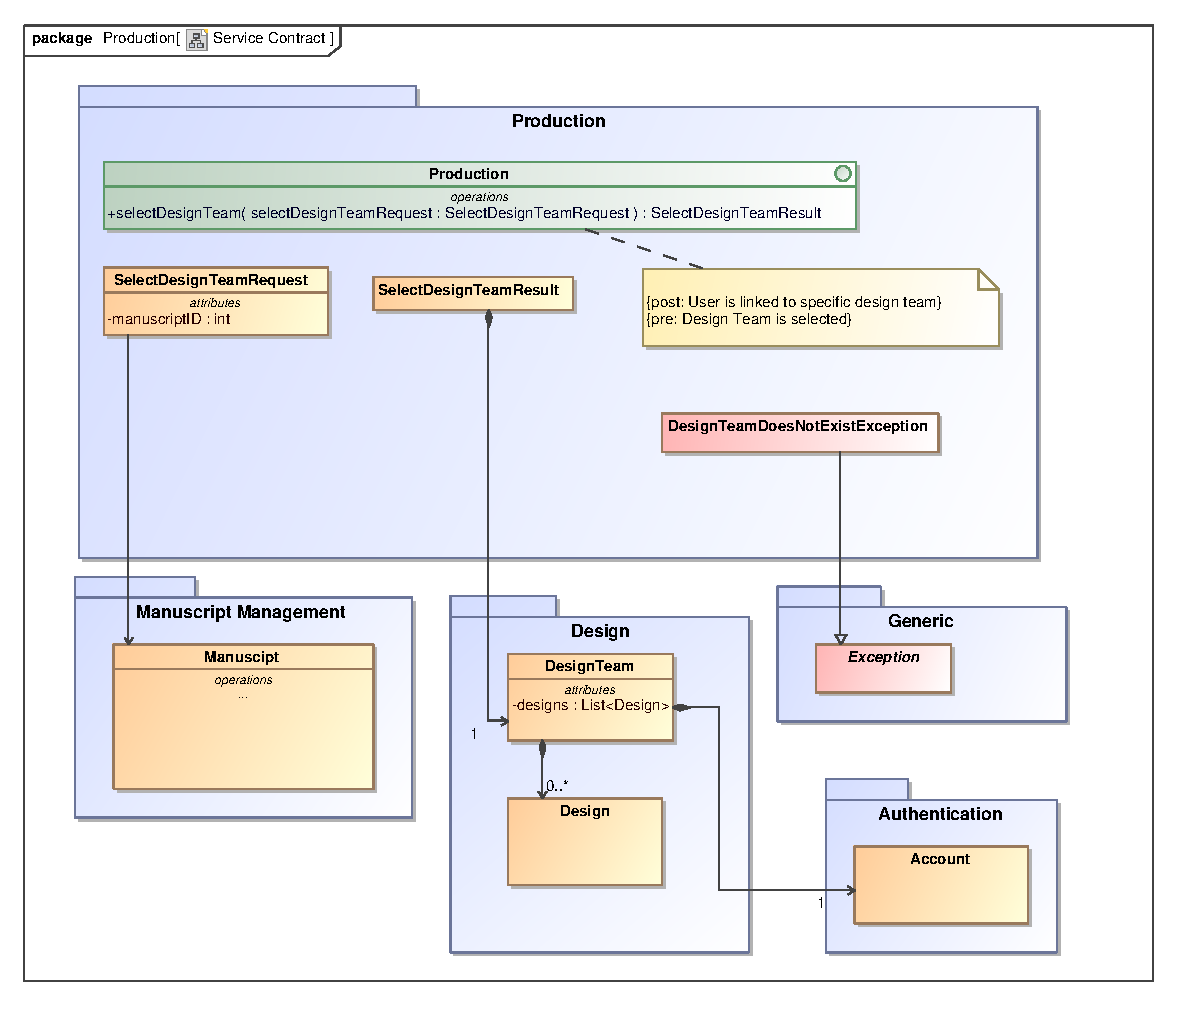
\includegraphics[height=380px, width=500px]{epsImages/Production/SelectDesignTeam.eps}
\caption{Service contract for selecting a design team}
\end{figure}


\newpage
\item \textbf{Publish - priority: critical}
\par{This use case allows an agent or an editorial to select a publisher and request that the final manuscript be published.}

\textbf{Service Contract:} 
The service contract for publish is shown in the diagram below. The pre-conditions are enforced (raising the appropriate exception should they not be met) and a preferred publisher is notified of the publishing request.

\begin{figure}[h]
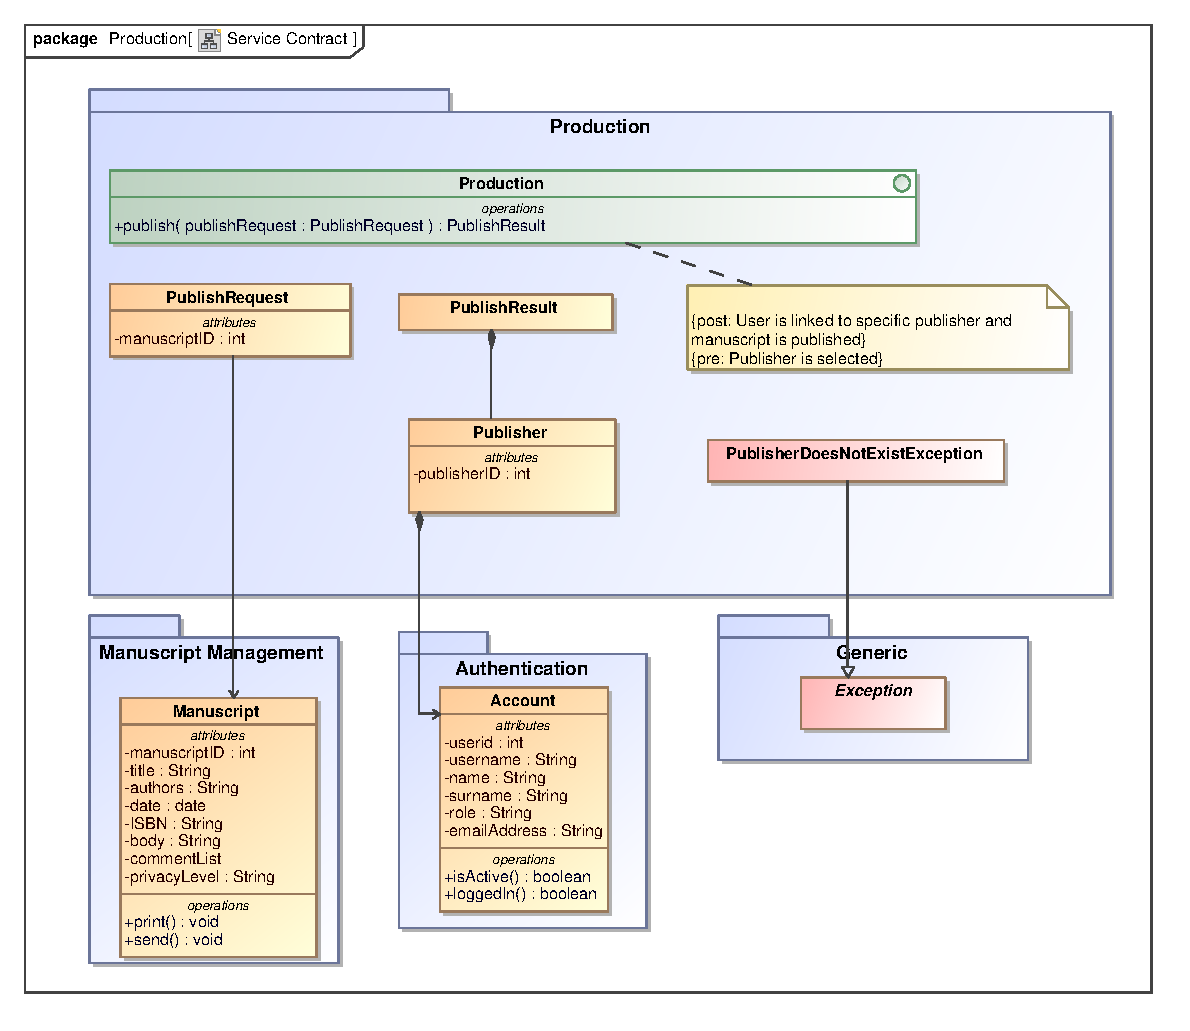
\includegraphics[height=380px, width=500px]{epsImages/Production/Publish.eps}
\caption{Service contract for evaluating a publish}
\end{figure}

 \newpage
\subsubsection{Domain Model}
\par{Production incorporates all the work that would generally be done by the publishing house. Everything from selecting the design team, to officially publishing the book with an ISBN number. All of which will be taken care of in this package.} 

\begin{figure}[h]
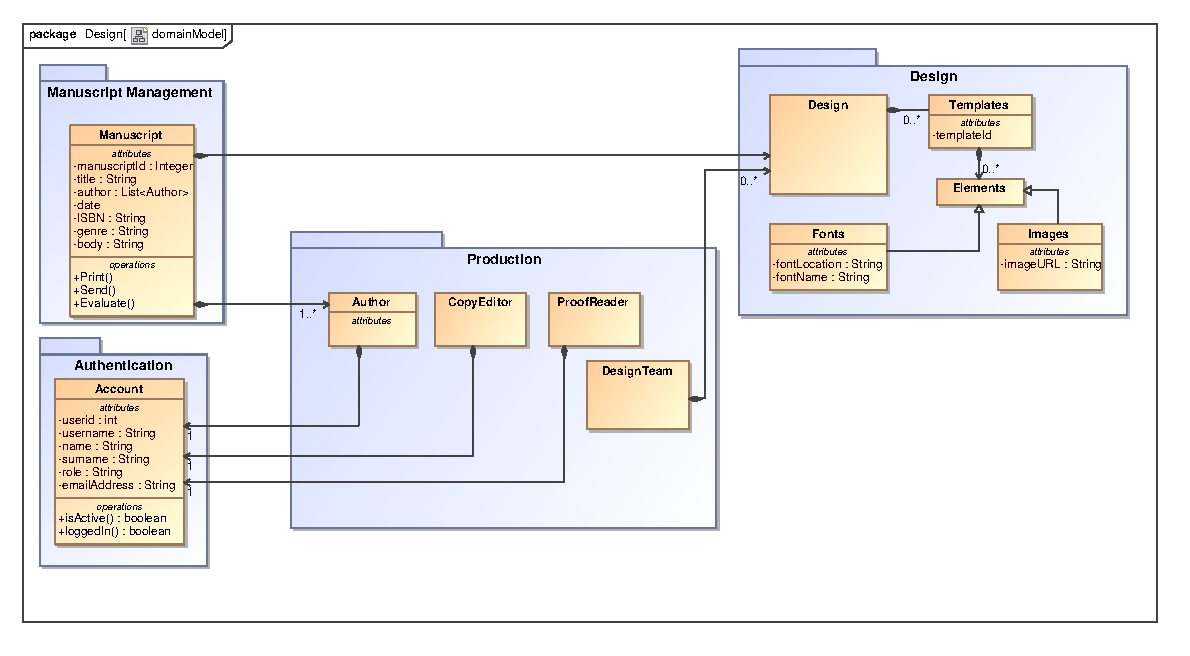
\includegraphics[height=380px, width=500px]{epsImages/DomainModels/ProductionDomainModel.eps}
\caption{Domain model for Production module}
\end{figure}


\end{enumerate}

\end{document}
